        %%******************************************%%
        %%                                          %%
        %%        Modello di tesi di laurea         %%
        %%            di Andrea Giraldin            %%
        %%                                          %%
        %%             2 novembre 2012              %%
        %%                                          %%
        %%******************************************%%

        \begin{document}
        \frontmatter
        \begin{titlepage}
    \begin{center}
        \begin{LARGE}
            \textbf{\myUni}\\
        \end{LARGE}

        \vspace{10pt}

        \begin{Large}
            \textsc{\myDepartment}\\
        \end{Large}

        \vspace{10pt}

        \begin{large}
            \textsc{\myFaculty}\\
        \end{large}

        \vspace{30pt}
        \begin{figure}[htbp]
            \centering
            
\includegraphics[height=6cm]{unipd-logo.png}
        \end{figure}
        \vspace{30pt}

        \begin{LARGE}
            \textbf{\myTitle}\\
        \end{LARGE}

        \vspace{10pt}

        \begin{large}
            \textsl{\myDegree}\\
        \end{large}

        \vspace{40pt}

        \begin{large}
            \begin{flushleft}
                \textit{Relatore}\\
                \vspace{5pt}
                \profTitle\ \myProf
            \end{flushleft}

            % You can tweak the spacing to have professor and student names on the same line
            % useful if the page is broken by a long thesis title and you need more space
            \vspace{-52pt}

            \begin{flushright}
                \textit{Laureando}\\
                \vspace{5pt}
                \myName \\
                \vspace{5pt}
                \textit{Matricola} \myID
            \end{flushright}
        \end{large}

        \vspace{40pt}

        \line(1, 0){338} \\
        \begin{normalsize}
            \textsc{Anno Accademico \myAA}
        \end{normalsize}
    \end{center}
\end{titlepage}

        \clearpage
\phantomsection
\thispagestyle{empty}

\hfill
\vfill

\noindent\myName: \textit{\myTitle,}
\myDegree,
\textcopyright\ \myTime.

        %%\cleardoublepage
\phantomsection
\thispagestyle{empty}
\pdfbookmark{Dedica}{Dedica}

\vspace*{3cm}

\begin{center}
    Lorem ipsum dolor sit amet, consectetuer adipiscing elit. \\ \medskip
    --- Oscar Wilde
\end{center}

\medskip

\begin{center}
    Dedicato a ...
\end{center}

        \cleardoublepage
\phantomsection
\pdfbookmark{Sommario}{Sommario}
\begingroup
\let\clearpage\relax
\let\cleardoublepage\relax
\let\cleardoublepage\relax

\chapter*{Sommario}

Il presente documento illustra il lavoro svolto dal laureando Cavalli Riccardo durante il periodo di stage interno presso l’Università degli Studi di Padova. Il tirocinio, della durata di circa 320 ore, è stato assegnato dalla Prof.ssa Ombretta Gaggi, con la collaborazione del Prof. Claudio Palazzi in qualità di tutor interno. Lo stage si è svolto nel periodo compreso tra il 7 aprile e il 9 giugno 2025.

\vspace{10pt}
\noindent Il progetto prevede lo sviluppo di uno strumento SEO per l’identificazione e l’analisi delle parole chiave all’interno di una pagina web. Le parole chiave possono essere estratte dal meta tag keywords (se presente), individuate automaticamente dal sistema in base a determinati criteri (come la frequenza), oppure inserite manualmente dall’utente. In aggiunta all’analisi delle parole chiave, questo strumento - da integrare in un’estensione per browser - deve anche consentire l’evidenziazione di tutte le occorrenze di una parola chiave nella pagina. La tesi descrive le fasi di sviluppo del progetto, seguendo i principi dell’ingegneria del software.

\vspace{10pt}
\noindent Il periodo di stage è stato suddiviso in tre fasi. La prima è stata dedicata allo studio delle soluzioni presenti sul mercato e alla stesura di una relazione sulle funzionalità, i vantaggi e gli svantaggi di ciascuno strumento, fornendo così una base per la formalizzazione dei requisiti. La seconda fase è stata riservata allo sviluppo delle funzionalità di analisi SEO. Infine, la terza fase è stata dedicata al collaudo del software.

%\vfill

%\selectlanguage{english}
%\pdfbookmark{Abstract}{Abstract}
%\chapter*{Abstract}

%\selectlanguage{italian}

\endgroup

\vfill

        %\cleardoublepage
\phantomsection
\pdfbookmark{Ringraziamenti}{ringraziamenti}

\begin{flushright}{
    \slshape
    ``No matter what anybody tells you, words and ideas can change the world''} \\
    \medskip
    --- Robin Williams (L'attimo fuggente)
\end{flushright}


\bigskip

\begingroup
\let\clearpage\relax
\let\cleardoublepage\relax
\let\cleardoublepage\relax

\chapter*{Ringraziamenti}

\textit{Innanzitutto, vorrei esprimere la mia gratitudine alla Prof.ssa \myProf{} per la guida e il supporto fornitomi durante lo svolgimento del progetto e la stesura della tesi, e in particolare per la disponibilità dimostrata fin dal primo incontro conoscitivo.}

\vspace{10pt}
\noindent \textit{Desidero ringraziare i miei genitori, Sabrina e Andrea, per avermi permesso di proseguire gli studi e per aver sempre sostenuto le mie scelte, giuste o sbagliate che fossero, senza le quali non sarei mai diventato la persona che oggi scrive queste parole.}

\vspace{10pt}
\noindent \textit{Ringrazio mio fratello Filippo, i miei nonni Elvia e Quinto, e tutti i parenti per l’interesse manifestato nei confronti del mio percorso universitario.}

\vspace{10pt}
\par\noindent \textit{Ringrazio gli amici con cui ho condiviso il percorso accademico per i bellissimi anni trascorsi insieme, scanditi da lunghissime sessioni di studio online, rilassanti viaggi in macchina nei giorni degli esami, attimi di gioia o di sconforto all’arrivo degli esiti, ma soprattutto da momenti di crescita personale che non dimenticherò mai.}

\vspace{10pt}
\noindent \textit{Ringrazio gli amici extra-universitari per esserci sempre stati, anche quando la mia attenzione nei loro confronti era totalmente assorbita dallo studio.}

\vspace{10pt}
\noindent \textit{Desidero infine ringraziare lo staff del multisala Metropolis Cinemas per l’impegno e la passione dedicati alla gestione del cinema del mio paese, luogo di tanti momenti indimenticabili.}

\bigskip

\noindent\textit{\myLocation, \myTime}
\hfill \myName

\endgroup

        \cleardoublepage
\pdfbookmark{\contentsname}{tableofcontents}
\setcounter{tocdepth}{3}
\setcounter{secnumdepth}{3}
\tableofcontents
%\markboth{\contentsname}{\contentsname}
\clearpage

\begingroup
    \let\clearpage\relax
    \let\cleardoublepage\relax
    \let\cleardoublepage\relax

    % Figures list
    \phantomsection
    \pdfbookmark{\listfigurename}{lof}
    \listoffigures

    \vspace*{8ex}

    % Tables list
    \phantomsection
    \pdfbookmark{\listtablename}{lot}
    \listoftables

    \vspace*{8ex}
\endgroup

\cleardoublepage

        \cleardoublepage
    
        \mainmatter
        \chapter{Analisi del contesto tecnologico}
\label{cap:analisi-soluzioni-esistenti}

\par Uno dei passi fondamentali nel processo di ottimizzazione \gls{seo} è la scelta delle parole chiave e il loro utilizzo in punti strategici delle pagine web. Esistono software in grado di automatizzare la ricerca e l'analisi delle parole chiave, contribuendo a migliorare il posizionamento e l'indicizzazione di un sito. Questi strumenti, disponibili gratuitamente o a pagamento, coprono numerosi aspetti dell'analisi \gls{seo}, tra cui:
\begin{itemize}
    \item Analisi \gls{seo} \gls{on-page} e \gls{off-page};
    \item Identificazione delle parole chiave più frequenti;
    \item Analisi della densità e della distribuzione delle parole chiave all'interno di una pagina web;
    \item Analisi dell'efficacia delle parole chiave;
    \item Ricerca delle parole chiave per cui un sito è posizionato in alto nella \gls{serp};
    \item Suggerimenti di parole chiave correlate e rilevanti;
    \item Anteprime \gls{serp} per una determinata parola chiave;
    \item Analisi dei \textit{competitor};
    \item Analisi di parametri come la \gls{keyword-difficulty} e di pratiche come il \gls{keyword-stuffing}.
\end{itemize}

\section{MozBar}

\subsection{Funzionalità}
\par \textit{MozBar} è un'estensione gratuita per Chrome che consente agli utenti di eseguire analisi \gls{seo} \gls{on-page} e \gls{off-page} senza aprire un'altra scheda del browser. Le funzionalità fornite dall'estensione includono:
\begin{itemize}
    \item \textbf{Page Authority e Domain Authority}: metriche da 1 a 100 che stimano il posizionamento di una singola pagina o di un dominio in base a un algoritmo di apprendimento automatico;
    \item \textbf{Linking Domains}: numero di domini unici che puntano a un sito;
    \item \textbf{Inbound Links}: numero di link in entrata provenienti da pagine web esterne;
    \item \textbf{Attributi generali}: tempo di caricamento, \gls{tag-canonical}, URL della cache di Google, \gls{sitemap}, \gls{hreflang}, \gls{tag-robots};
    \item \textbf{Elementi on-page}: URL, titolo, meta description, meta tag keywords, elenco degli heading, testo alternativo delle immagini;
    \item \textbf{Dati strutturati (\gls{json-ldg})}: verifica che lo schema sia formattato correttamente;
    \item \textbf{Ranking Keywords}: identifica le parole chiave per cui un sito è posizionato e fornisce informazioni sui \textit{competitor};
    \item \textbf{Ottimizzazione della pagina}: visualizza il punteggio ottenuto per una determinata parola chiave e mostra  i fattori che contribuiscono al punteggio complessivo, nonché quelli che potrebbero danneggiarlo;
    \item \textbf{Highlight links}: evidenzia tutte le tipologie di link presenti all'interno della pagina;
    \item \textbf{Highlight keywords}: questa funzionalità, rappresentata in figura \ref{fig:mozbar}, consente agli utenti di inserire una parola chiave e ottenere il numero di occorrenze. Inoltre, permette di evidenziare graficamente una parola chiave all'interno della pagina.
\end{itemize}

\begin{figure}[H]
    \centering 
    \fbox{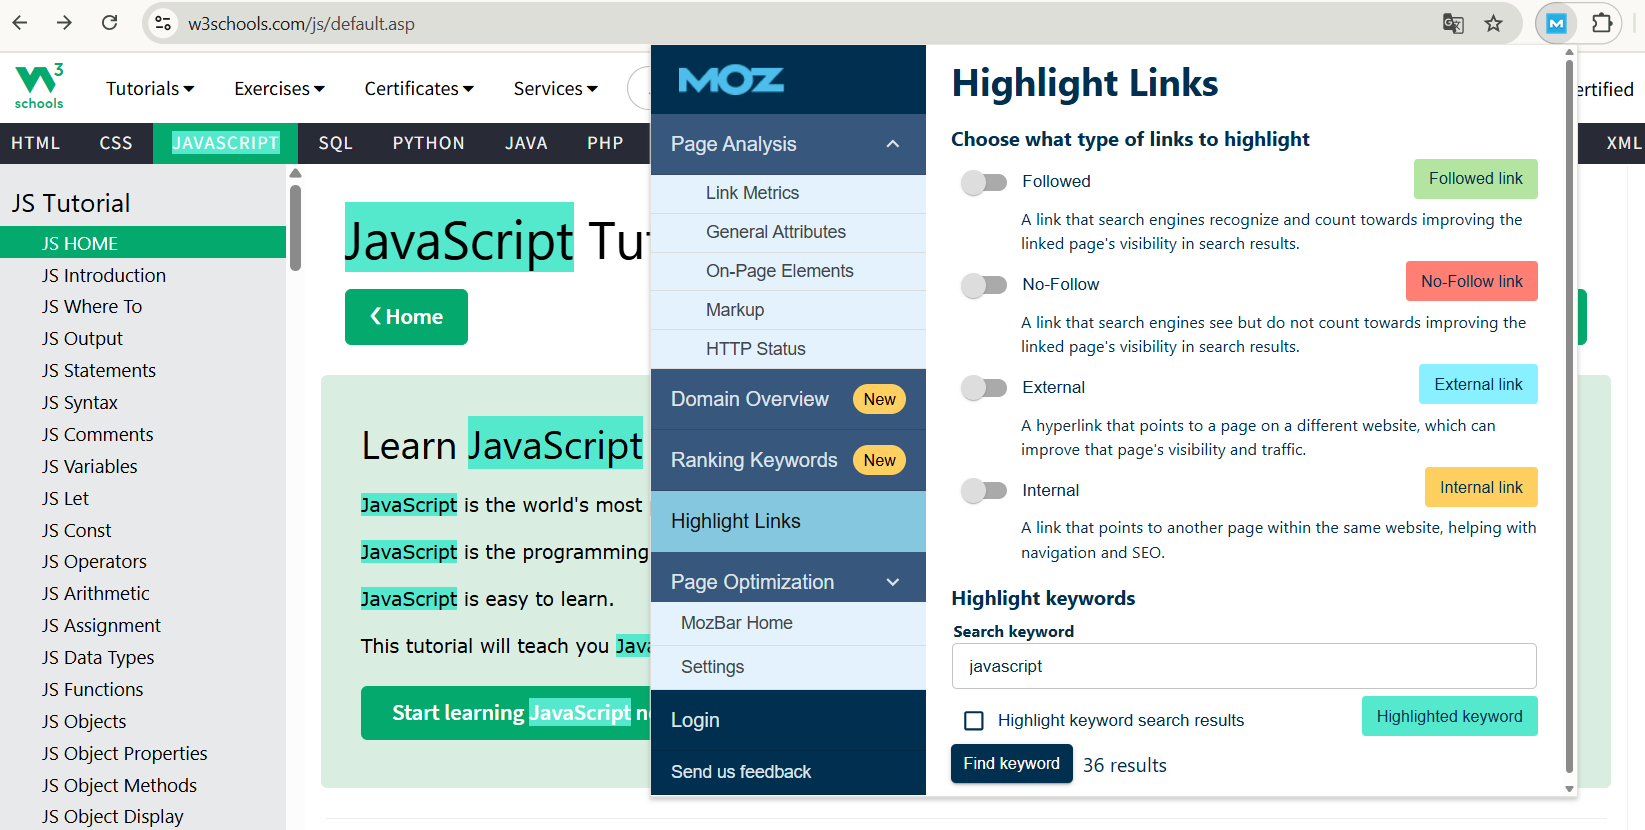
\includegraphics[width=0.9\columnwidth]{soluzioni-esistenti/MozBar/moz_bar_search_keywords.png}}
    \caption{MozBar - Analisi del sito “W3Schools”}
    \label{fig:mozbar}
\end{figure}

\subsection{Vantaggi}
\par Poiché funziona su \gls{localhost}, l'estensione può essere facilmente usata durante lo sviluppo. La barra degli strumenti può essere ancorata in alto o in basso nella pagina e le metriche \gls{seo} possono essere visualizzate direttamente nei risultati di ricerca.

\subsection{Svantaggi}
\par L'estensione non è disponibile come barra laterale, ma solo come pop-up o barra degli strumenti. L'analisi delle parole chiave non include alcuni aspetti essenziali, come la densità o la distribuzione. Inoltre, il rilevamento dei tag è \gls{case-sensitive}, quindi c'è il rischio che alcuni tag non vengano individuati se si usa la lettera iniziale maiuscola. Le funzionalità Premium richiedono un abbonamento a pagamento. 

\section{Wincher}

\subsection{Funzionalità}
\par \textit{Wincher} è una piattaforma orientata alla ricerca e all'analisi delle parole chiave; in particolare, \textit{Wincher} monitora il posizionamento di un sito web, i volumi di ricerca, il traffico stimato e le anteprime \gls{serp}. La piattaforma include anche l'\textit{On-Page SEO Checker}, uno strumento di analisi \gls{on-page} per un URL e una parola chiave specifici. Il \textit{tool}, rappresentato in figura \ref{fig:on_page_seo_checker}, fornisce suggerimenti per migliorare una pagina web in relazione alla parola chiave scelta:
\begin{itemize}
    \item \textbf{Titolo}: lunghezza del titolo, presenza e posizione della parola chiave nel titolo;
    \item \textbf{Heading}: lunghezza e numero di occorrenze del tag H1, presenza e posizione della parola chiave nel tag H1, differenza di contenuto tra il titolo e il tag H1, presenza della parola chiave nei sottotitoli;
    \item \textbf{Meta}: presenza della parola chiave nel meta tag description;
    \item \textbf{Media}: presenza della parola chiave nel testo alternativo delle immagini;
    \item \textbf{URL}: presenza della parola chiave negli URL;
    \item \textbf{Body}: la parola chiave dovrebbe essere menzionata almeno tre volte nel corpo del testo.
\end{itemize}

\begin{figure}[H]
    \centering 
    \fbox{
\includegraphics[width=0.8\columnwidth]{soluzioni-esistenti/Wincher/wincher_seo_checker.png}}
    \caption{Wincher - On-Page SEO Checker}
    \label{fig:on_page_seo_checker}
\end{figure}

\subsection{Vantaggi}
\par \textit{On-Page SEO Checker} fornisce un punteggio complessivo e dei suggerimenti per garantire la conformità di una pagina alle attuali linee guida \gls{seo}.

\subsection{Svantaggi}
\par Lo strumento di analisi \gls{on-page} non funziona su \gls{localhost} ed è accessibile esclusivamente tramite la piattaforma di \textit{Wincher}. Nella versione gratuita, i controlli giornalieri sono limitati.

\vspace{10pt}
\par\noindent La figura \ref{fig:wincher_w3schools} mostra un esempio di analisi del sito “W3Schools” effettuata con \textit{Wincher}.

\begin{figure}[H]
    \centering 
    \fbox{
\includegraphics[width=0.8\columnwidth]{soluzioni-esistenti/Wincher/wincher_seo_checker_score.png}}
    \caption{Wincher - Analisi del sito “W3Schools”}
    \label{fig:wincher_w3schools}
\end{figure}

\section{SEOquake}

\subsection{Funzionalità}
\par \textit{SEOquake} è un plugin che fornisce metriche \gls{seo} e strumenti di analisi \gls{on-page}. Le parole chiave vengono identificate tramite un algoritmo di ricerca e successivamente elencate in quattro tabelle distinte:
\begin{itemize}
    \item Keyword di 1 parola;
    \item Keyword di 2 parole;
    \item Keyword di 3 parole;
    \item Keyword di 4 parole.
\end{itemize}
\vspace{5pt}
\par\noindent Per ogni parola chiave, \textit{SEOquake} visualizza il numero di occorrenze e la densità. Inoltre, verifica se ciascuna parola chiave appare nei seguenti tag \gls{html}:
\begin{itemize}
    \item Titolo della pagina;
    \item Meta description;
    \item Meta tag keywords;
    \item Tag H1.
\end{itemize}
\vspace{5pt}
\par\noindent Tutti questi fattori contribuiscono a determinare un punteggio di importanza per ogni parola chiave. \textit{SEOquake} permette anche di filtrare le parole chiave, esportare i risultati dell'analisi in formato \gls{csv} e configurare un elenco di parole da includere o escludere. La figura \ref{fig:seoquake_w3schools} mostra un esempio di analisi del sito “W3Schools” effettuata con \textit{SEOquake}.

\begin{figure}[H]
    \centering 
    \fbox{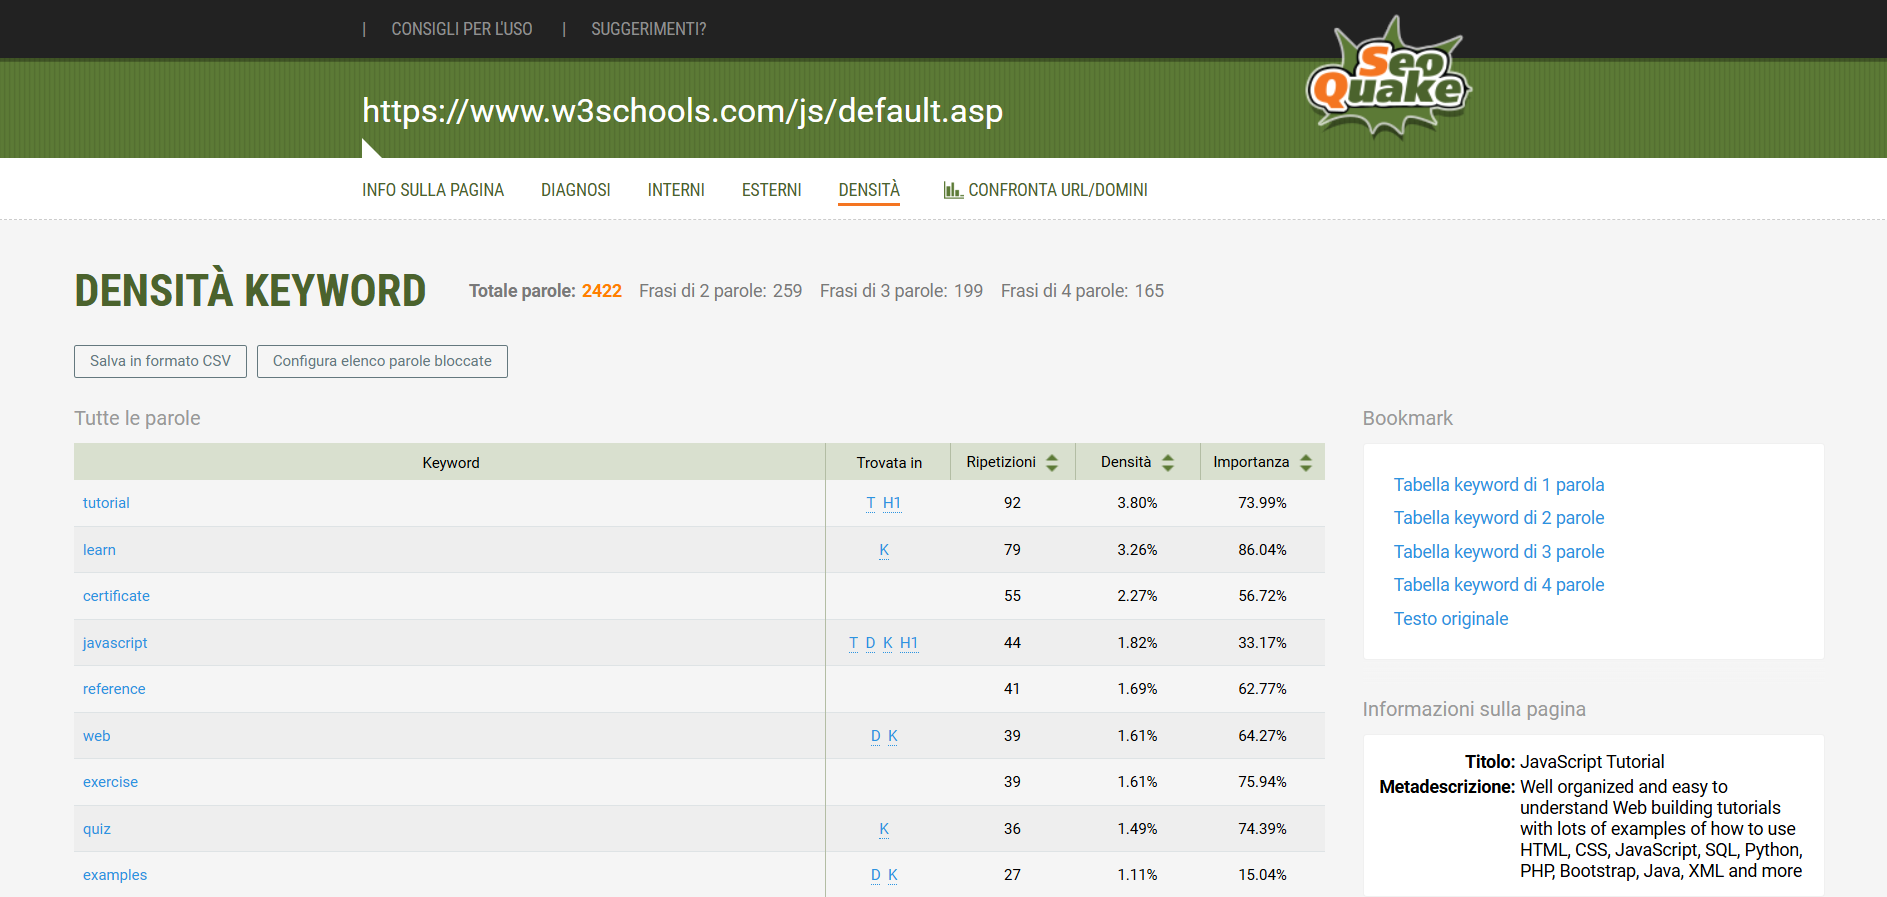
\includegraphics[width=0.9\columnwidth]{soluzioni-esistenti/SEOquake/seoquake.png}} 
    \caption{SEOquake - Analisi del sito “W3Schools”}
    \label{fig:seoquake_w3schools}
\end{figure}

\subsection{Vantaggi}
\par Oltre all'analisi \gls{on-page}, \textit{SEOquake} offre anche funzionalità avanzate come l'analisi dei \gls{backlink} e del traffico; il tutto è integrato in un'unica piattaforma che funziona su \gls{localhost}. L'estensione è sviluppata da \textit{Semrush} e, pertanto, include servizi propri della piattaforma.

\subsection{Svantaggi}
\par Le funzionalità di analisi \gls{seo} \gls{on-page} sono accessibili solo tramite la \textit{dashboard} esterna, il che limita l'interazione diretta con la pagina corrente.

\section{SEOptimer}

\subsection{Funzionalità}
\par \textit{SEOptimer} è una piattaforma di analisi \gls{seo} e reportistica. Offre una suite completa di strumenti che coprono le seguenti funzionalità:
\begin{itemize}
    \item \textbf{Audit SEO}: fornisce un punteggio complessivo basato su fattori come \gls{seo} \gls{on-page} e \gls{off-page}, usabilità, performance e ottimizzazione per i social media;
    \item \textbf{Crawler SEO}: esegue una scansione dettagliata di una pagina web, includendo un'analisi della distribuzione delle parole chiave. Le parole chiave vengono estratte in base alla frequenza e suddivise in:
    \begin{itemize}
        \item Keyword di 1 parola;
        \item Keyword di 2 o più parole.
    \end{itemize}
    Le parole chiave dovrebbero essere distribuite correttamente tra i seguenti tag \gls{html}: 
    \begin{itemize}
        \item Titolo della pagina;
        \item Meta description;
        \item Tag di intestazione (heading).
    \end{itemize}
    \item \textbf{Monitoraggio delle parole chiave};
    \item \textbf{Ricerca di parole chiave}: analizza i \textit{competitor} e fornisce suggerimenti per nuove parole chiave;
    \item \textbf{Ricerca e monitoraggio dei \gls{backlink}}.
\end{itemize}

\vspace{10pt}
\par\noindent La figura \ref{fig:seoptimer_w3schools} mostra un esempio di analisi del sito “W3Schools” effettuata con \textit{SEOptimer}.

\begin{figure}[H]
    \centering 
    \fbox{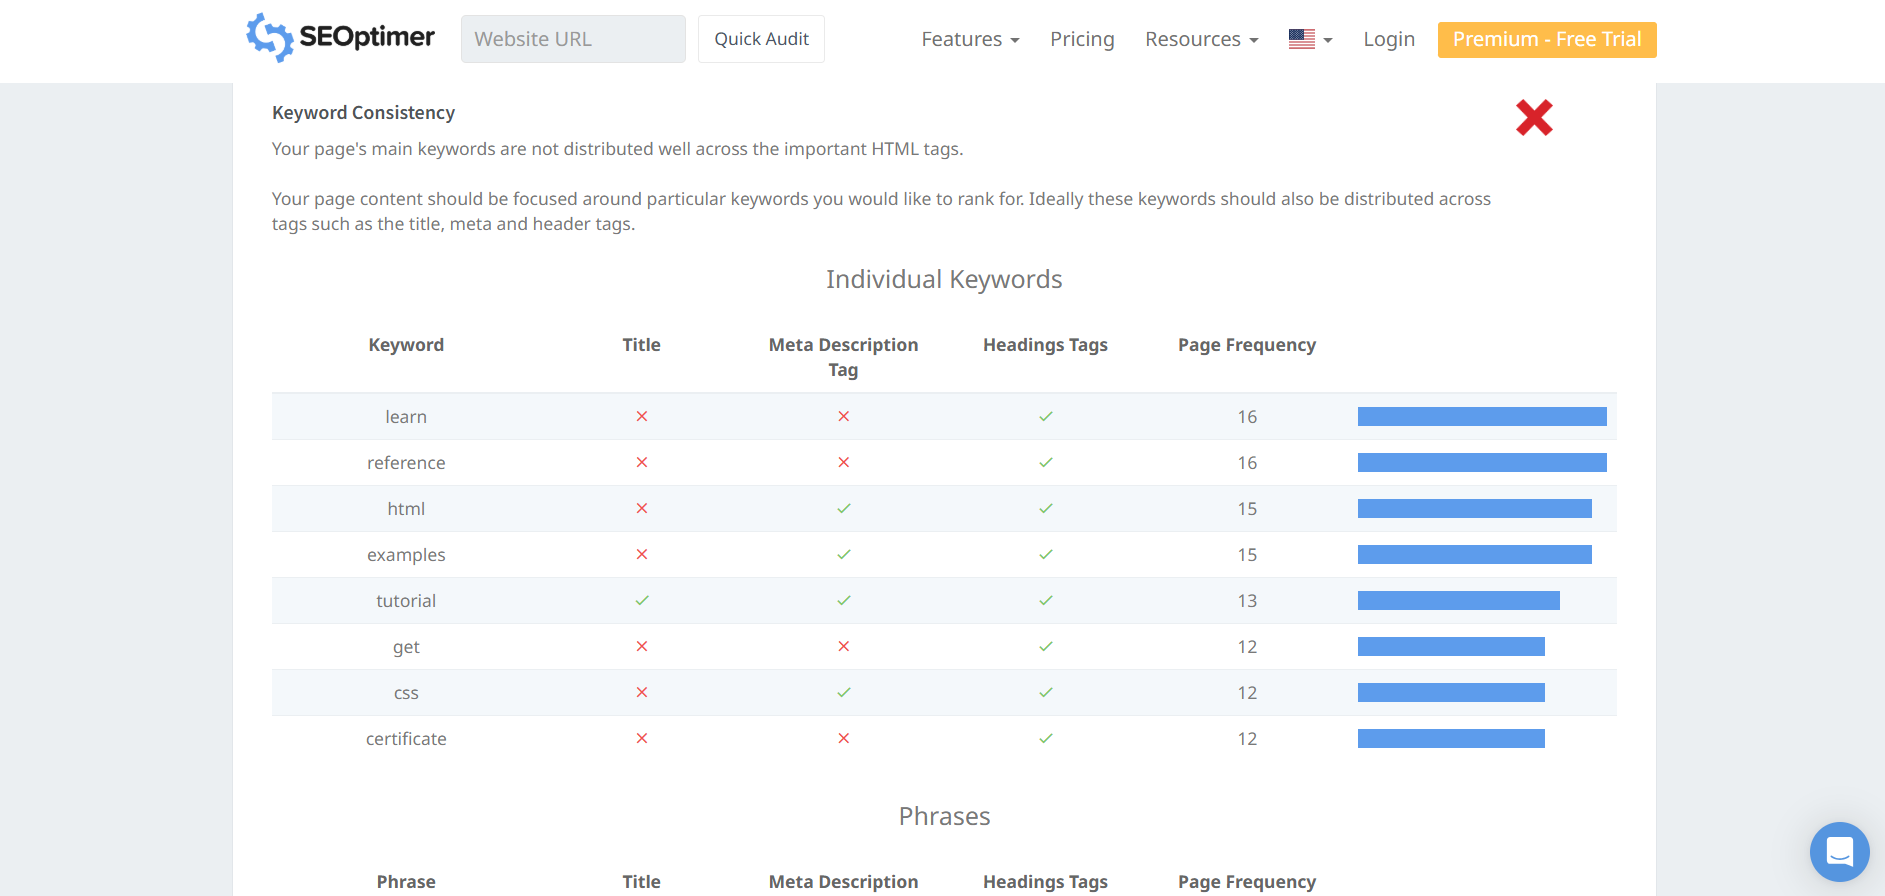
\includegraphics[width=0.9\columnwidth]{soluzioni-esistenti/SEOptimer/seoptimer.png}} 
    \caption{SEOptimer - Analisi del sito “W3Schools”}
    \label{fig:seoptimer_w3schools}
\end{figure}

\subsection{Vantaggi}
\par \textit{SEOptimer} integra in un'unica piattaforma tutti gli strumenti necessari per un'analisi \gls{seo} approfondita ed è più economico rispetto ad altri servizi simili.

\subsection{Svantaggi}
\par \textit{SEOptimer} non funziona su \gls{localhost} e la versione gratuita consente un numero limitato di report giornalieri. Non è disponibile un'estensione per browser, pertanto l'analisi può essere eseguita soltanto tramite la piattaforma proprietaria.

\section{SEO tester online}

\subsection{Funzionalità}
\par \textit{SEO tester online} è un'estensione gratuita per Chrome sviluppata da \textit{Sitechecker}. Fornisce una panoramica generale dei dati \gls{seo} essenziali, seguita da un elenco di sezioni specifiche, tra cui:
\begin{itemize}
    \item \textbf{Contenuto}: analizza la gerarchia degli heading, la lunghezza del testo, il rapporto testo/codice \gls{html} e la densità delle keyword composte da 1, 2 o 3 parole;
    \item \textbf{Link e immagini};
    \item \textbf{\Gls{hreflang} e dati strutturati};
    \item \textbf{Velocità di caricamento};
    \item \textbf{Analisi \gls{gsc}}.
\end{itemize}

\subsection{Vantaggi}
\par L'estensione è gratuita e si integra con \gls{gsc}, offrendo un'analisi \gls{seo} completa e professionale.

\subsection{Svantaggi}
\par L'estensione non funziona su \gls{localhost} e si apre unicamente come pop-up.

\vspace{10pt}
\par\noindent La figura \ref{fig:seo_tester_online_w3schools} mostra un esempio di analisi del sito “W3Schools” effettuata con \textit{SEO tester online}.

\begin{figure}[H]
    \centering 
    \fbox{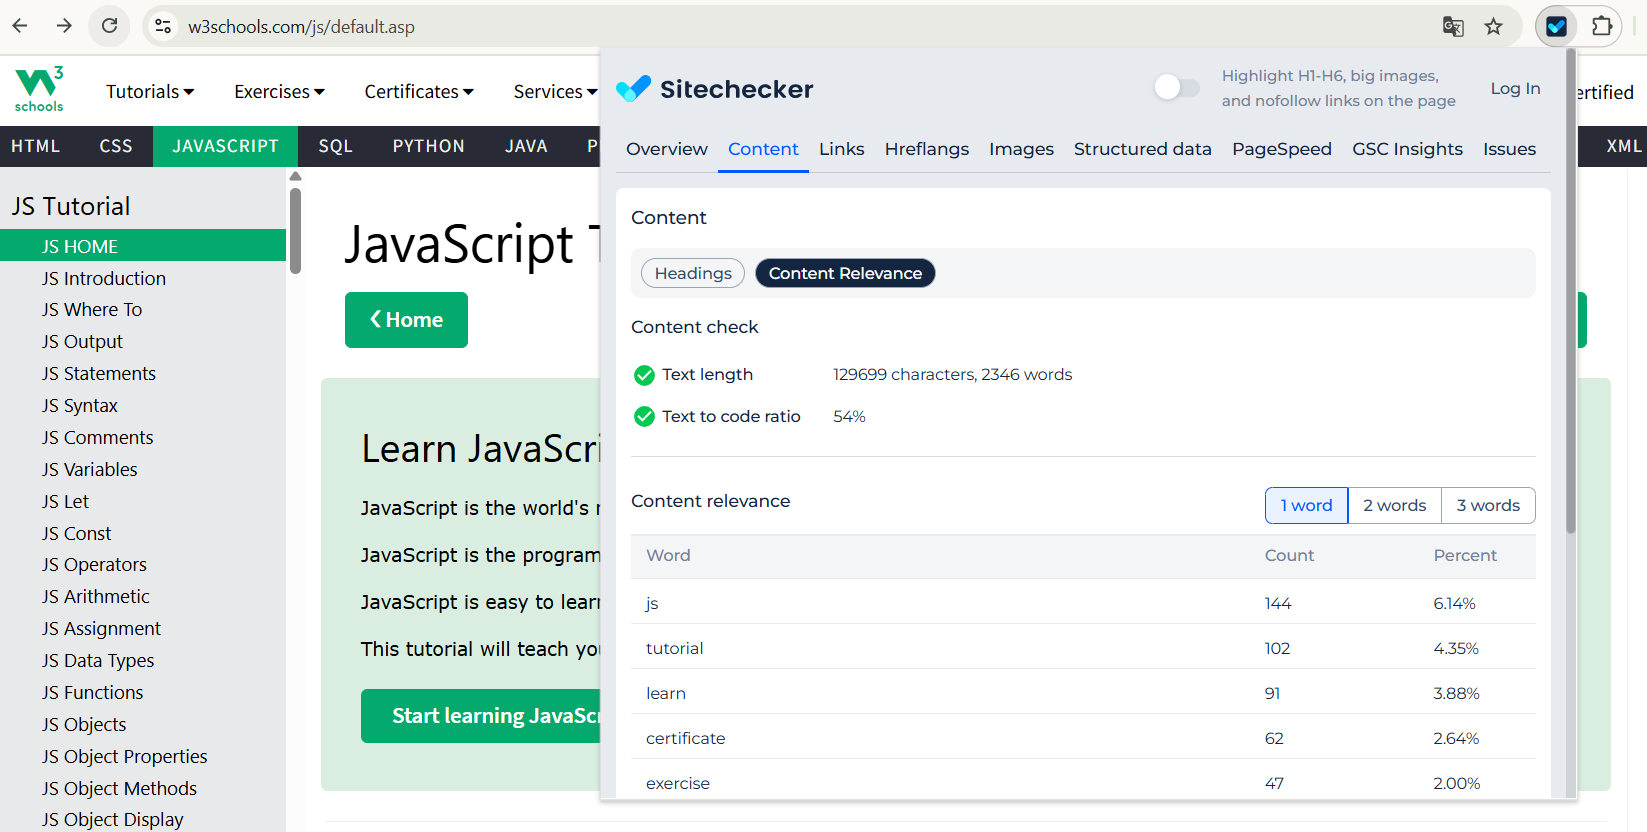
\includegraphics[width=0.9\columnwidth]{soluzioni-esistenti/SEO-Tester-Online/site_checker.png}} 
    \caption{SEO tester online - Analisi del sito “W3Schools”}
    \label{fig:seo_tester_online_w3schools}
\end{figure}

\section{Semrush}

\subsection{Funzionalità}
\par \textit{Semrush} include oltre 50 strumenti di analisi \gls{seo}, il che lo rende una delle piattaforme più complete sul mercato. La \textit{dashboard}, mostrata in figura \ref{fig:semrush}, consente di visualizzare gratuitamente analisi relative al traffico, ai \gls{backlink}, alle ricerche \gls{organiche} e a quelle \gls{sponsorizzate}. In merito all’analisi delle parole chiave, \textit{Semrush} offre le seguenti funzionalità:
\begin{itemize}
    \item \textbf{Analisi SEO on-page};
    \item \textbf{Keyword research}: suggerisce parole chiave rilevanti in base al volume di ricerca, all'intento, alla \gls{keyword-difficulty} e ad altri fattori \gls{seo}. Questa funzionalità può essere integrata con plugin di terze parti, tra cui \textit{Yoast SEO} per \gls{wordpress};
    \item \textbf{Analisi dei competitor};
    \item \textbf{Position tracking}: monitora il posizionamento nella \gls{serp} per determinate parole chiave.
\end{itemize}

\begin{figure}[H] 
    \centering 
    \fbox{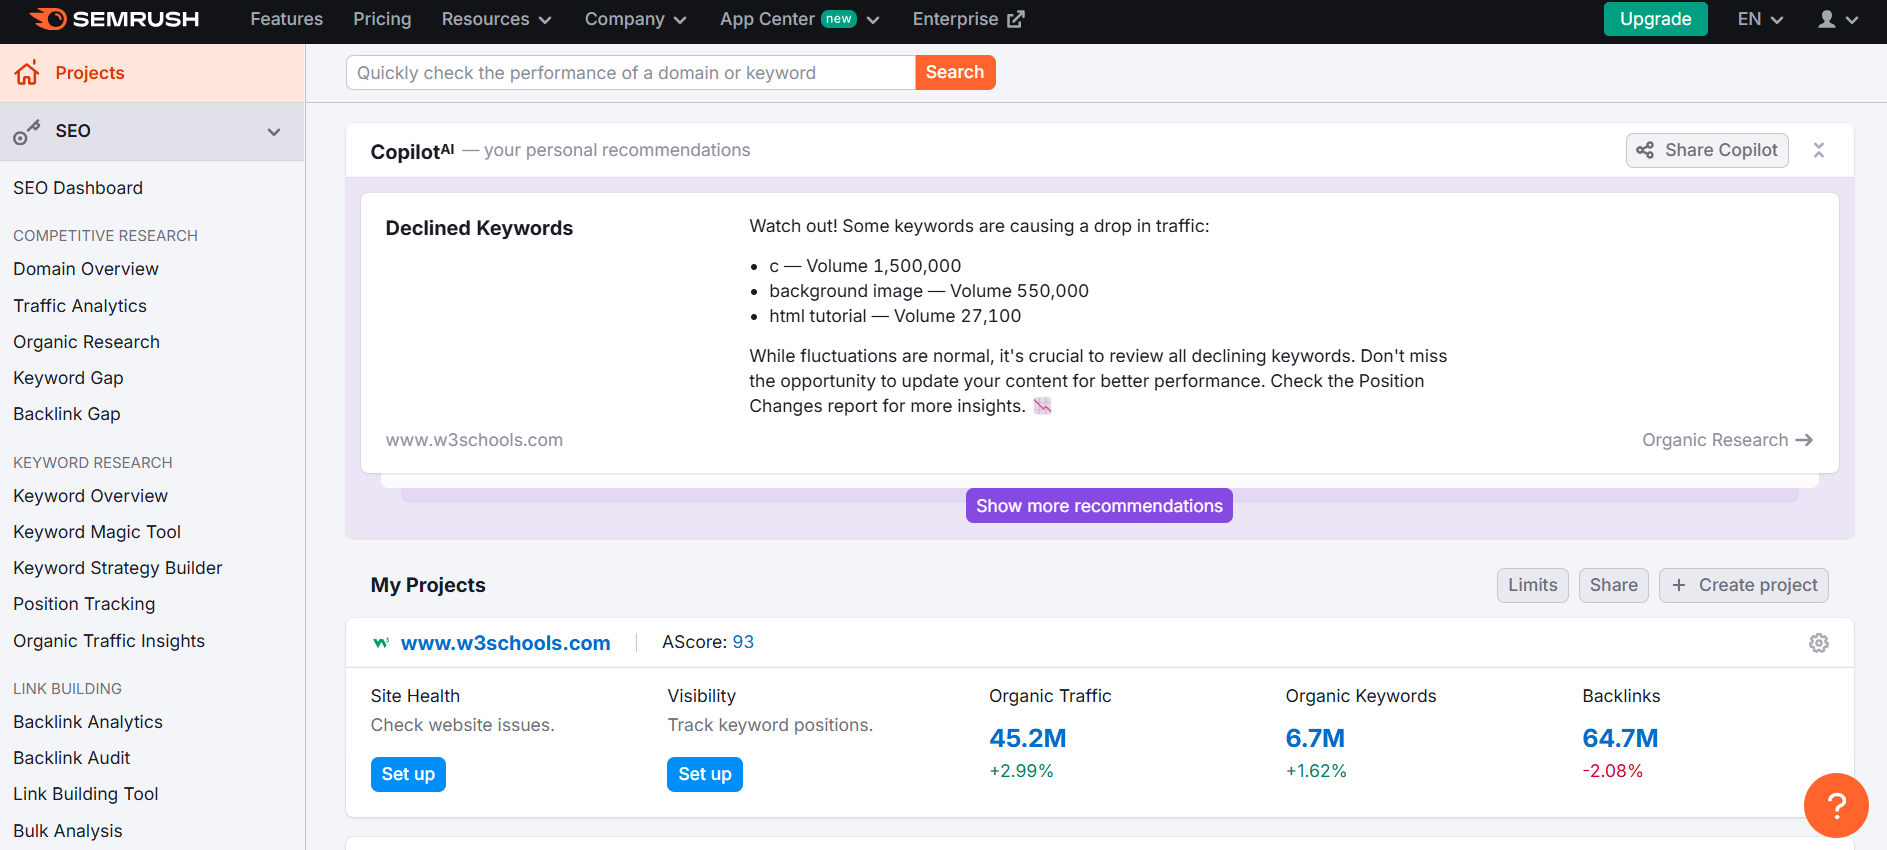
\includegraphics[width=0.8\textwidth]{soluzioni-esistenti/SEMrush/semrush.png}} 
    \caption{Semrush - SEO dashboard}
    \label{fig:semrush}
\end{figure}

\subsection{Vantaggi}
\par \textit{Semrush} può essere integrato facilmente con altri strumenti di analisi \gls{seo}.

\subsection{Svantaggi}
\par Le funzionalità avanzate sono a pagamento. Per effettuare un'analisi, è necessario interrompere la navigazione e accedere alla piattaforma web di \textit{Semrush}.

\section{Yoast SEO (plugin per CMS)}

\subsection{Funzionalità}
\par \textit{Yoast SEO} è un plugin per \gls{cms} che semplifica il processo di ottimizzazione \gls{seo}. Fornisce feedback in tempo reale per migliorare il posizionamento sui motori di ricerca. La versione del plugin per \gls{wordpress} consente di ottimizzare le parole chiave (note anche come keyphrase) attraverso un'analisi della densità, della distribuzione e di altri fattori \gls{on-page}. Con la versione a pagamento, l'utente può anche scegliere manualmente delle keyphrase correlate (argomenti collegati o parole chiave secondarie) da valutare distintamente. Inoltre, l'integrazione con \textit{Semrush} fornisce automaticamente suggerimenti di keyphrase correlate basati sui volumi di ricerca, sull'intento e sulla \gls{keyword-difficulty}. Naturalmente, i controlli sono meno restrittivi rispetto alla keyphrase principale. Per evitare di dover ripetere meccanicamente la stessa keyphrase, la versione Premium permette anche di aggiungere uno o più sinonimi, che \textit{Yoast} interpreta allo stesso modo senza penalizzare il punteggio.

\subsection{Vantaggi}
\par \textit{Yoast SEO} è disponibile in versione gratuita per \gls{wordpress}, seppur con alcune limitazioni, e può essere integrato con altri strumenti come \textit{Semrush} e \textit{Wincher}. Il plugin viene aggiornato regolarmente per rimanere allineato agli algoritmi dei motori di ricerca e alle \textit{best practice} \gls{seo}.

\subsection{Svantaggi}
\par \textit{Yoast SEO} è limitato a \gls{cms} come \gls{wordpress} e \gls{shopify}. Alcune funzionalità, tra cui l'inserimento di keyphrase correlate e sinonimi, o l'integrazione con \textit{Semrush}, richiedono la sottoscrizione di un abbonamento a pagamento.

\vspace{10pt}
\par\noindent La figura \ref{fig:yoast_seo} mostra un esempio di analisi effettuata con \textit{Yoast SEO Premium}.

\begin{figure}[H]
    \centering 
    \fbox{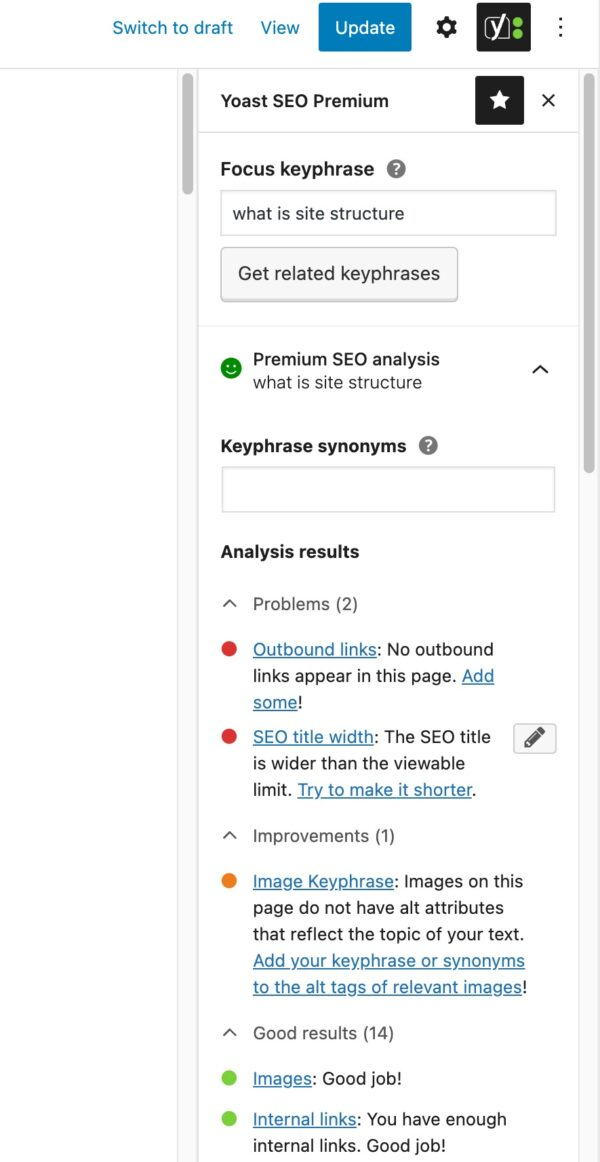
\includegraphics[width=0.4\columnwidth]{soluzioni-esistenti/Yoast-SEO/yoast_seo_premium.png}} 
    \caption{Yoast SEO Premium - Analisi SEO}
    \label{fig:yoast_seo}
\end{figure}

\section{Keyword Density Analyzer}

\subsection{Funzionalità}
\par \textit{Keyword Density Analyzer} è uno strumento di analisi \gls{seo} fornito da \textit{Webmaster Tips}. L'analisi inizia con una panoramica generale della pagina esaminata, che include le seguenti informazioni:
\begin{itemize}
    \item URL, titolo, meta description e lingua;
    \item Dimensione della pagina non compressa;
    \item Dimensione del contenuto di testo semplice;
    \item Rapporto testo semplice/codice \gls{html};
    \item Conteggio di caratteri e parole;
    \item \textbf{Top keywords}: elenco delle parole chiave considerate più rilevanti in base a parametri interni all'applicazione.
\end{itemize}
\vspace{5pt}
\par\noindent Viene poi effettuata un'analisi del titolo e della meta description, evidenziando la frequenza e la densità di ciascuna parola contenuta in questi tag. L'analisi delle parole chiave è suddivisa in quattro sezioni:
\begin{itemize}
    \item \textbf{Meta tag keywords}: mostra la frequenza e la densità delle parole chiave specificate nel meta tag keywords;
    \item \textbf{Top Keywords by Density}: elenca le parole più frequenti, escludendo quelle comuni e troppo brevi. Oltre alla frequenza e alla densità, mostra anche il numero di occorrenze nel titolo, negli heading, nei link e nel testo alternativo delle immagini;
    \item \textbf{Top Keywords by Score}: elenca le parole in base a un punteggio calcolato internamente, come mostrato in figura \ref{fig:keyword_density_analyzer};
    \item \textbf{Top Phrases}: elenca le frasi con più di una occorrenza, escludendo quelle brevi e con parole comuni.
\end{itemize}

\vspace{10pt}
\par\noindent La figura \ref{fig:keyword_density_analyzer_w3schools} mostra un esempio di analisi del sito “W3Schools” effettuata con \textit{Keyword Density Analyzer}.

\begin{figure}[H]
    \centering 
    \fbox{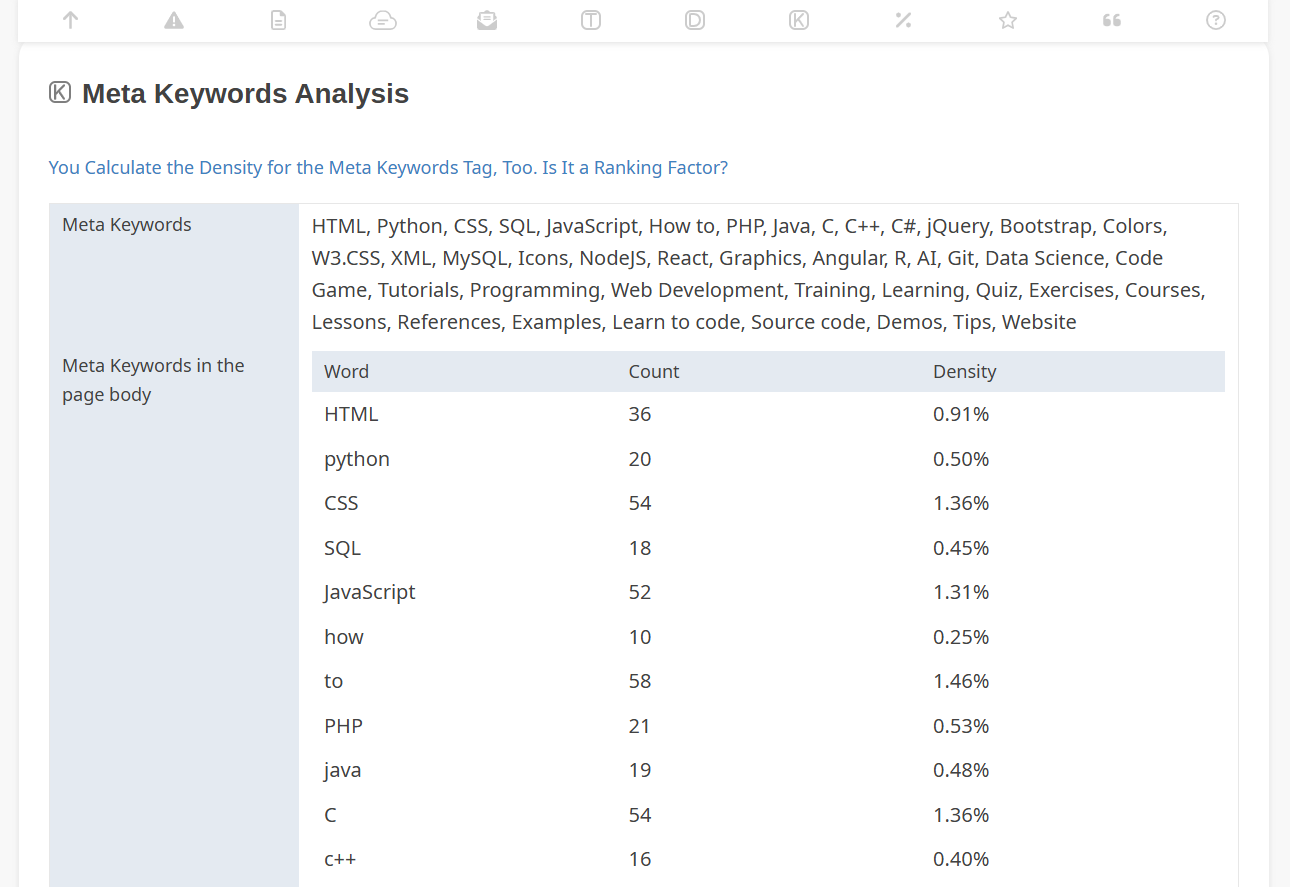
\includegraphics[width=0.8\columnwidth]{soluzioni-esistenti/Keywords-Density-Analyzer/keywords_density_analyzer.png}} 
    \caption{Keyword Density Analyzer - Analisi del sito “W3Schools”}
    \label{fig:keyword_density_analyzer_w3schools}
\end{figure}

\subsection{Vantaggi}
\par Tutte le funzionalità sono gratuite e possono essere integrate con gli altri strumenti di \textit{Webmaster Tips} per un'analisi \gls{seo} completa.

\subsection{Svantaggi}
\par L'analisi di una pagina web richiede di interrompere la navigazione e accedere alla piattaforma di \textit{Webmaster Tips}.

\begin{figure}[H]
    \centering 
    \fbox{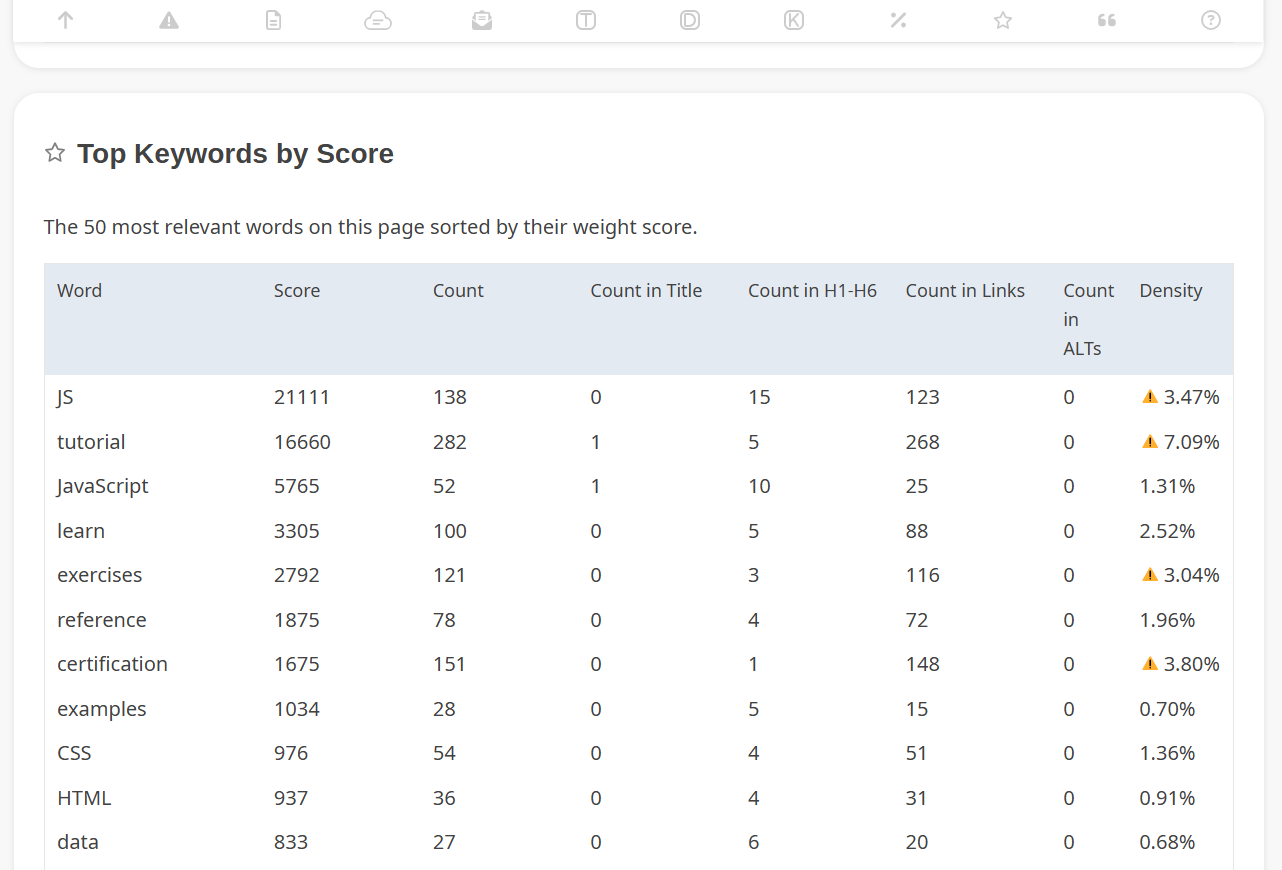
\includegraphics[width=0.8\columnwidth]{soluzioni-esistenti/Keywords-Density-Analyzer/keywords_density_analyzer_score.png}} 
    \caption{Keyword Density Analyzer - Top Keywords by Score}
    \label{fig:keyword_density_analyzer}
\end{figure}

\section{Detailed SEO Extension}

\subsection{Funzionalità}
\par \textit{Detailed SEO Extension} è un'estensione per Google Chrome e Firefox che consente di analizzare, con un solo clic, qualsiasi sito web. L'estensione estrae e analizza i seguenti elementi:
\begin{itemize}
    \item \textbf{Overview}: Titolo, meta description, URL, \gls{tag-canonical}, \gls{tag-robots}, meta tag keywords, numero di parole e lingua;
    \item \textbf{Gerarchia degli heading} (da H1 a H6): l'estensione regola l'indentazione e la dimensione del font in base al livello, facilitando l'analisi visiva della struttura;
    \item \textbf{Link} (unici, interni o esterni, completi o incompleti);
    \item \textbf{Immagini} (complete o prive di attributi);
    \item \textbf{Schema e \gls{hreflang}};
    \item \textbf{Ottimizzazione per i social media}.
\end{itemize}
\vspace{5pt}
\par\noindent Inoltre, l'estensione genera automaticamente i link per analizzare la stessa pagina web su altre piattaforme, tra cui \textit{Ahrefs}, \textit{Majestic}, \textit{Moz}, \textit{Semrush} e \textit{SimilarWeb}. La figura \ref{fig:detailed_seo_extension_w3schools} mostra un esempio di analisi del sito “W3Schools” effettuata con \textit{Detailed SEO Extension}.
 
\begin{figure}[H]
    \centering 
    \fbox{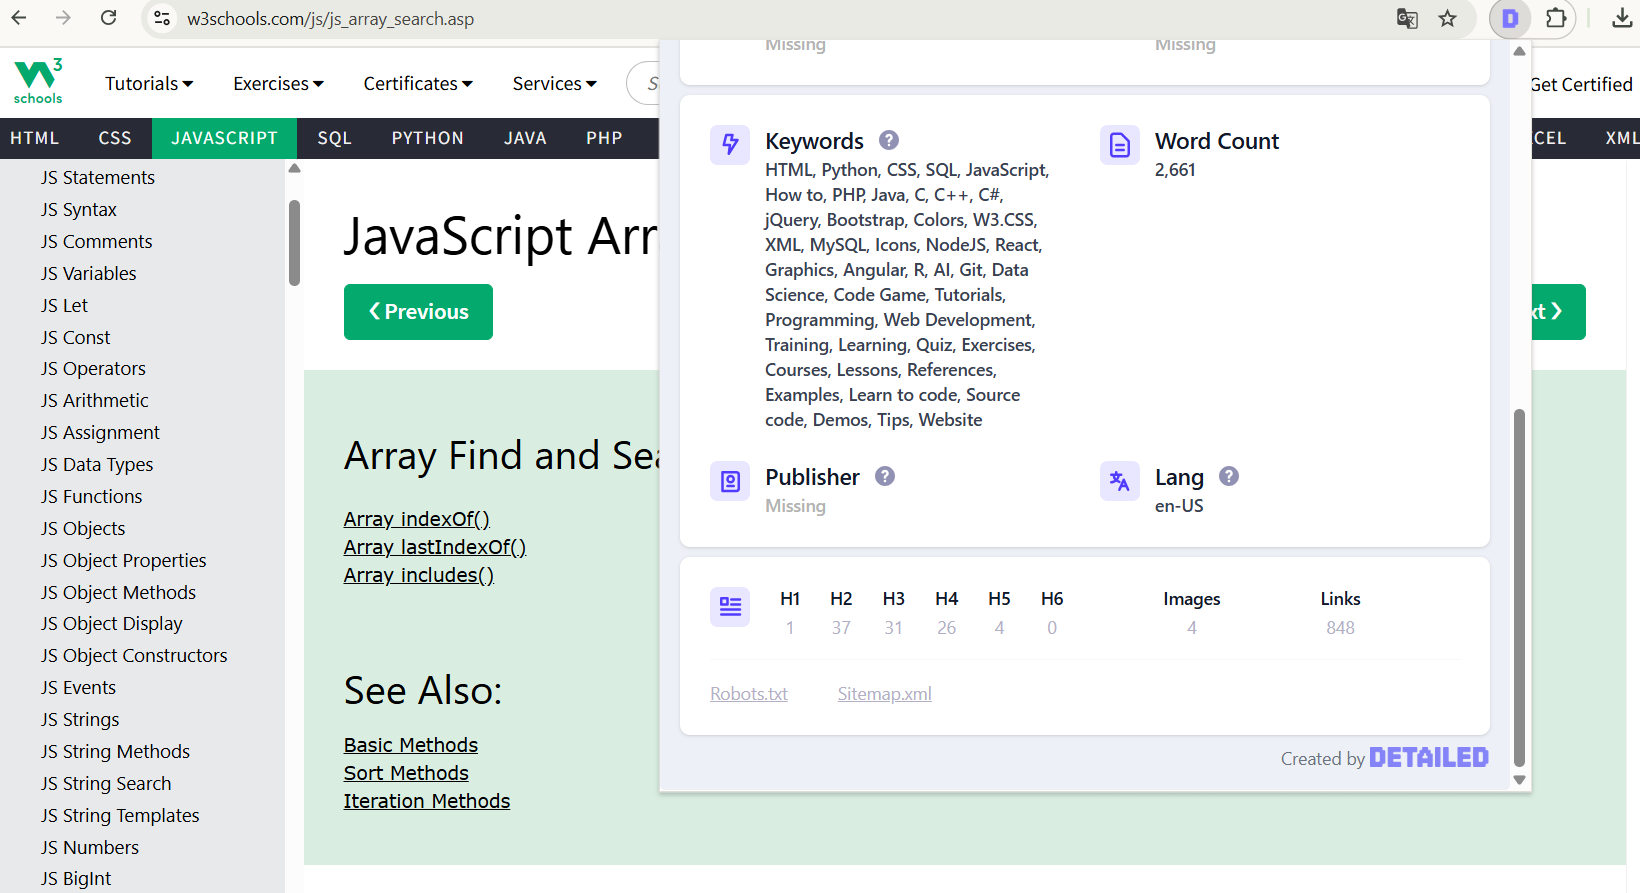
\includegraphics[width=0.8\columnwidth]{soluzioni-esistenti/Detailed-SEO-Extension/detailed_seo_analysis.png}} 
    \caption{Detailed SEO Extension - Analisi del sito “W3Schools”}
    \label{fig:detailed_seo_extension_w3schools}
\end{figure}

\subsection{Vantaggi}
\par Essendo gratuita e compatibile con \gls{localhost}, l'estensione si presta perfettamente all'uso durante la fase di sviluppo.

\subsection{Svantaggi}
\par L'estensione si apre come pop-up, il che può rendere meno agevole l'interazione con la pagina corrente. Per quanto riguarda l'analisi delle parole chiave, lo strumento si limita a estrarre quelle presenti nel meta tag keywords.

\section{SEO Analyzer (Rank Math)}

\subsection{Funzionalità}
\par \textit{Rank Math} è un plugin per \gls{wordpress} che semplifica l'ottimizzazione \gls{seo} mediante suggerimenti basati sulle \textit{best practice}. Lo strumento \textit{SEO Analyzer} esegue un'analisi approfondita delle pagine web, generando un punteggio complessivo. Inoltre, \textit{SEO Analyzer} visualizza un elenco delle parole chiave più frequenti e verifica che siano distribuite correttamente.

\subsection{Vantaggi}
\par \textit{SEO Analyzer} è in grado di analizzare anche siti web che non sono stati realizzati con \gls{wordpress}.

\subsection{Svantaggi}
\par \textit{SEO Analyzer} non funziona su \gls{localhost} ed è meno affidabile rispetto ad altri strumenti, in quanto l'analisi dei tag è \gls{case-sensitive}, il che può portare a errori come il mancato rilevamento della meta description. Inoltre, la versione Premium di \textit{Rank Math} è a pagamento. 

\vspace{10pt}
\par\noindent La figura \ref{fig:rank_math_silktide} mostra un esempio di analisi del sito “Silktide” effettuata con \textit{Rank Math}.

\begin{figure}[H]
    \centering 
    \fbox{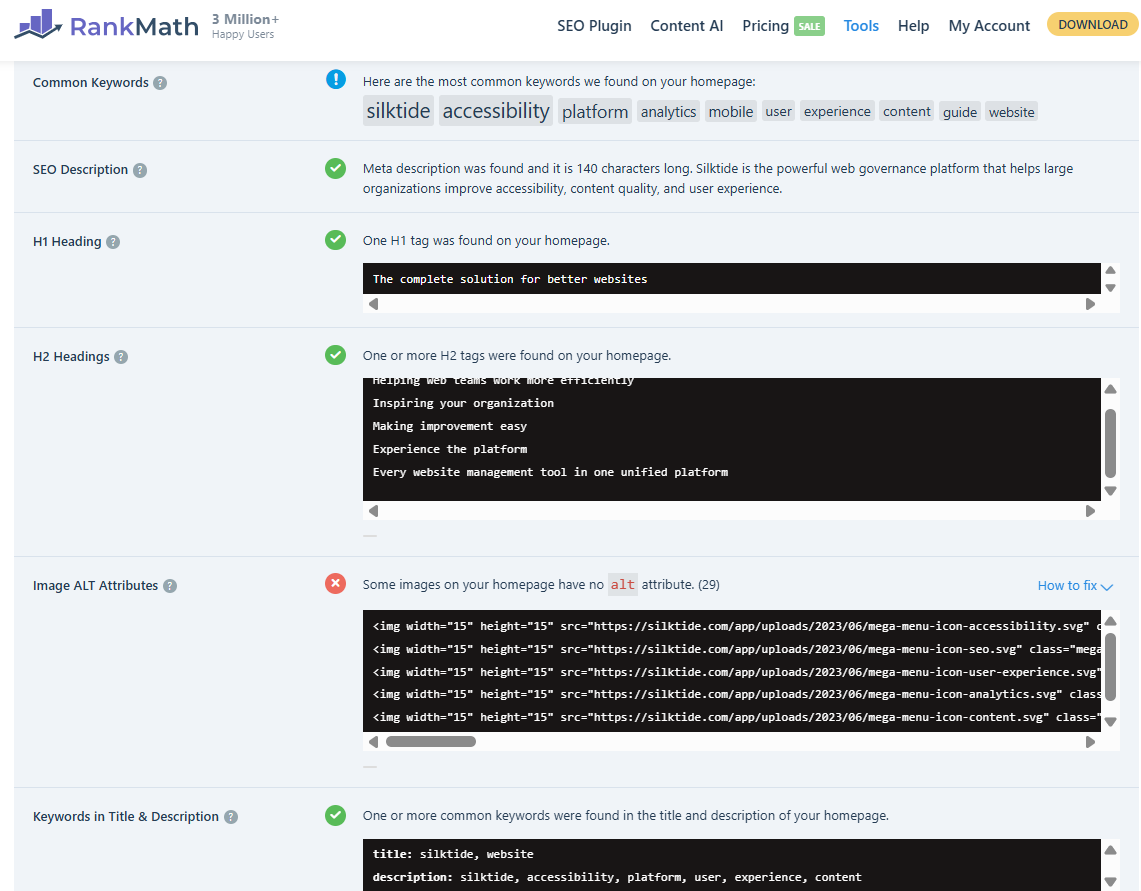
\includegraphics[width=0.7\columnwidth]{soluzioni-esistenti/RankMath/rank_math.png}} 
    \caption{Rank Math - Analisi del sito “Silktide”}
    \label{fig:rank_math_silktide}
\end{figure}
        %\chapter{Introduzione}
\label{cap:introduzione}

\par Uno degli obiettivi principali di chi pubblica contenuti sul web è garantirne la massima visibilità. In altri termini, sviluppatori, redattori e altre figure professionali operanti nel settore digitale mirano a ottenere un buon posizionamento nella \gls{serp}, affinché i propri contenuti possano raggiungere il pubblico più ampio possibile. In un panorama in cui gli ambiti e le aree di maggiore interesse per l’utenza sono già ampiamente coperti, realizzare un sito accattivante e ricco di funzionalità non è più sufficiente. Ritagliarsi uno spazio in un mercato saturo è ancora possibile, ma comporta uno sforzo significativo in termini di risorse e competenze, legato principalmente al processo di ottimizzazione \gls{seo}.

\vspace{10pt}
\par\noindent Per “ottimizzazione SEO” si intende l’insieme di strategie e tecniche finalizzate ad aumentare la visibilità di una pagina web. I motori di ricerca, in risposta a una \textit{query} dell’utente, generano un elenco di risultati organici (non a pagamento), che include collegamenti alle pagine ritenute più pertinenti in base a molteplici fattori. L’obiettivo dell’ottimizzazione SEO è migliorare il posizionamento di una pagina all’interno di questo elenco, incrementando così le probabilità che venga visitata dagli utenti.

\vspace{10pt}
\par\noindent I risultati restituiti dai motori di ricerca sono strutturati secondo un sistema di paginazione. Numerosi studi evidenziano come gli utenti attribuiscano maggiore credibilità ai siti collocati nelle primissime posizioni della SERP, ignorando quasi del tutto quelli che compaiono nelle pagine successive. Le strategie SEO si suddividono in due macro-aree: \gls{on-page} e \gls{off-page}. Tra i fattori on-page che influenzano il \textit{ranking}, rivestono particolare importanza la scelta delle parole chiave e il loro utilizzo in punti strategici della pagina.

\section{La Proponente}

\par Il progetto di stage, svolto internamente all’Università degli Studi di Padova, è stato commissionato dalla Prof.ssa Ombretta Gaggi, che ha ricoperto il ruolo di tutor esterno. Si tratta di un progetto accademico continuativo, avviato nel 2024 nell’ambito di un tirocinio, finalizzato allo sviluppo di un’estensione web orientata all’accessibilità e all’ottimizzazione \gls{seo}.

\section{L'idea}

\par Ai fini dell’ottimizzazione \gls{seo}, l’inserimento delle parole chiave in sezioni strategiche della pagina risulta fondamentale. Con il termine “sezioni strategiche” si intendono elementi \gls{html} particolarmente rilevanti in ottica SEO, tra cui:
\begin{itemize}
    \item Il tag title;
    \item La meta description;
    \item I tag di intestazione (heading);
    \item Il testo alternativo delle immagini.
\end{itemize}

\vspace{5pt}
\par\noindent Una volta selezionate le parole chiave, verificarne la presenza nelle aree strategiche e analizzarne la distribuzione all’interno del \gls{dom} sono operazioni complesse, ripetitive e dispendiose se svolte manualmente. Da qui nasce l’opportunità - approfondita nel \hyperref[cap:descrizione-progetto]{capitolo successivo} - di sviluppare un’estensione web che automatizzi tale processo.

\section{Glossario}

\par Allo scopo di evitare incomprensioni legate al linguaggio utilizzato, è stato inserito, in calce al documento, un glossario in cui ogni termine è corredato da una spiegazione volta a illustrarne il significato. Oltre a termini ambigui o poco comuni, il glossario include anche acronimi e abbreviazioni. La prima occorrenza di ciascun termine è evidenziata con la seguente formattazione: \textit{termine}\glsfirstoccur.

\section{Convenzioni tipografiche}

\par Relativamente alla stesura del testo, sono state adottate le seguenti convenzioni tipografiche:
\begin{itemize}
	\item Il \textit{corsivo} è utilizzato per termini tecnici, espressioni in lingua straniera e voci del glossario alla loro prima occorrenza;
	\item Il \textbf{grassetto} è riservato esclusivamente alle intestazioni o ai concetti su cui si intende porre una forte enfasi;
	\item Nel corpo del testo vengono utilizzate unicamente le virgolette alte doppie (“...”).
\end{itemize}

        %\chapter{Processi e metodologie}
\label{cap:processi-metodologie}

\intro{In questa sezione viene illustrato l’approccio organizzativo adottato per il progetto, includendo le strategie implementate per automatizzare i processi.}

\section{Modello di sviluppo}

\par L’organizzazione del lavoro è stata gestita tramite la piattaforma Jira, utilizzando un template \textit{Kanban} semplificato. Questo modello fornisce una \textit{timeline}, una \textit{board} suddivisa nelle etichette “Da completare”, “In corso” e “Completato” (analogamente a Trello), un calendario e una \textit{dashboard} per monitorare l’integrazione con \gls{github}. Il progetto è stato suddiviso in tre \textit{epic}, o macro-fasi (analisi, sviluppo, validazione), ciascuna delle quali si è conclusa con il rilascio di un prodotto. Ogni rilascio di documentazione o software è stato associato a una specifica \textit{milestone}. Il tempo dedicato ai tre \textit{epic} è stato ulteriormente articolato in periodi settimanali (simili agli \textit{sprint} della metodologia \textit{agile}). Questo approccio ha permesso di mantenere un rapporto costante con la Proponente; al termine di ogni periodo è stato fornito un aggiornamento sullo stato di avanzamento, in presenza o da remoto (tramite comunicazione via e-mail), e sono state pianificate le attività successive. La priorità delle attività è stata concordata settimanalmente con la Proponente, così da definire un elenco ordinato (simile a un \textit{backlog}) di \textit{task} da completare entro la fine dell’iterazione.

\section{Workflow GitHub}

\par Per gestire lo sviluppo, ho adottato una struttura basata su due \textit{branch} principali: \textit{main} e \textit{develop}. Il \textit{branch main} registra la cronologia dei rilasci e contiene codice stabile, pronto per la produzione, mentre \textit{develop} rappresenta la linea di sviluppo principale. A ciascuna funzionalità da implementare è associato un \textit{branch} dedicato, contraddistinto dal prefisso \textit{feature/}, che ne accompagna lo sviluppo fino all’integrazione in un ramo condiviso. Quando una funzionalità risulta completa o pronta per l’integrazione, viene sottoposta a revisione tramite l’apertura di una \gls{pull request}, che può essere arricchita con commenti, etichette, \textit{issue} e \textit{milestone}.

\vspace{10pt}
\par\noindent Questo flusso di lavoro è riconducibile al modello \textit{Gitflow}, introdotto da Vincent Driessen nel 2010. Nell’ambito del progetto di stage, il modello \textit{Gitflow} non è stato applicato in modo rigido, ma ibridato con alcuni principi dello sviluppo \textit{trunk-based}. Idealmente, \textit{Gitflow} prevede \textit{branch} isolati e di lunga durata, mentre l’approccio \textit{trunk-based} favorisce aggiornamenti piccoli e frequenti, anche in assenza del completamento di una funzionalità, sfruttando appieno il potenziale della \gls{continuous integration}.

\vspace{10pt}
\par\noindent Per avviare il rilascio di una nuova versione, \textit{Gitflow} prevede la creazione di un \textit{branch} con il prefisso \textit{release/}. Il rilascio vero e proprio si concretizza con l’integrazione nel \textit{branch main}, che viene contrassegnato con un numero di versione. La versione può essere etichettata come “latest” oppure “pre-release”, qualora non sia ancora pronta per l’ambiente di produzione. Al termine del rilascio, i due \textit{branch} principali, \textit{main} e \textit{develop}, devono essere riallineati.

\section{Workflow Jira}

\par Prima di creare un branch su \gls{github}, a ciascuna funzionalità viene associato un \textit{ticket}, che può essere arricchito con commenti, etichette, date di inizio e fine, ed eventuali sotto-ticket. La creazione del \textit{branch} può avvenire direttamente da Jira, così da garantire un collegamento automatico con il relativo \textit{ticket}. In alternativa, il collegamento tra un \textit{ticket} e un \textit{branch}, un \gls{commit} o una \gls{pull request} può essere stabilito inserendo l’ID del \textit{ticket} come commento. Se l’ID viene racchiuso tra parentesi quadre (es. [ID]) all’interno della sezione commenti di una \gls{pull request}, il \textit{bot} di Jira genera automaticamente un collegamento ipertestuale al progetto.

\section{Automatizzazione dei processi}

\par Ho configurato un \textit{workflow}, tramite \textit{GitHub Actions}, che si attiva a ogni apertura, aggiornamento o chiusura di una \gls{pull request}. Il \textit{workflow}, scritto in \gls{yaml}, avvia due \textit{job} principali: l’esecuzione dei test automatizzati e il monitoraggio della \textit{code coverage}. Per i test è stato adottato il \gls{framework} Jest, che produce automaticamente un report sulla copertura del codice. Il report viene inviato a Codecov, che aggiorna la \textit{dashboard} del progetto, genera un \textit{badge} di stato e pubblica un riepilogo nei commenti della \gls{pull request}. Il superamento dei test e il mantenimento della copertura (rispetto alla versione precedente) rappresentano condizioni necessarie per procedere con il \textit{merge}. Questo approccio promuove la \gls{continuous integration} e fornisce una valutazione oggettiva della qualità del codice.

\vspace{10pt}
\par\noindent Su Jira ho definito tre regole di automazione:
\begin{itemize}
  \item \textbf{PR\_merged}: si attiva quando viene eseguito il \textit{merge} di una \gls{pull request} e sposta i \textit{ticket} collegati dallo stato corrente a “Completato”;
  \item \textbf{TICKET\_closed}: si attiva quando tutti i \textit{ticket} subordinati risultano completati e sposta l'elemento principale dallo stato corrente a “Completato”;
  \item \textbf{TICKET\_reopened}: si attiva quando un \textit{ticket} subordinato viene (ri)aperto e sposta l’elemento principale dallo stato “Completato” a “In corso”.
\end{itemize}

\begin{figure}[H] 
  \centering 
  \fbox{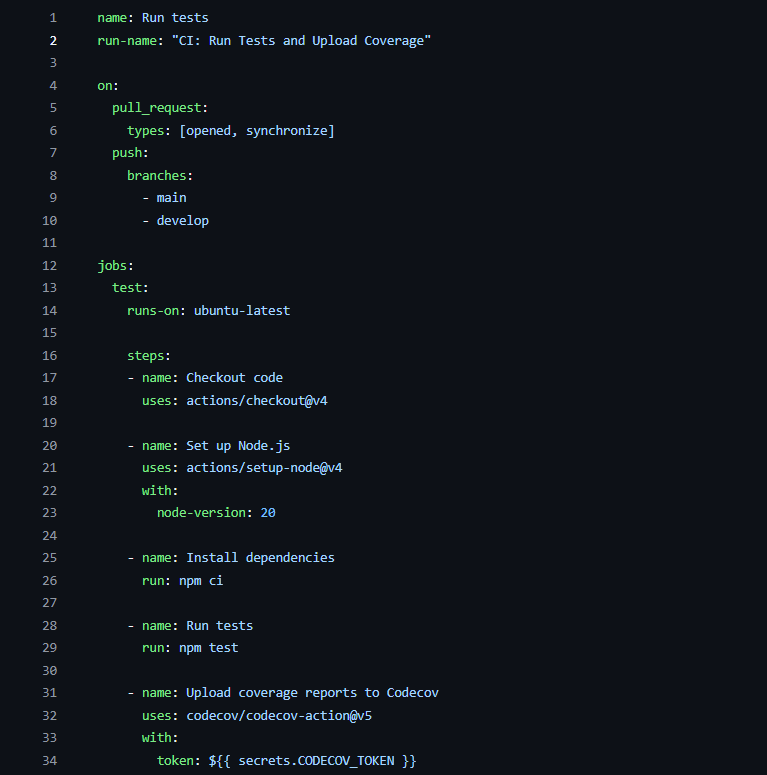
\includegraphics[width=0.9\textwidth]{processi/workflow.png}}
  \caption{Workflow YAML per continuous integration}
\end{figure}
        %\chapter{Descrizione dello stage}
\label{cap:descrizione-stage}

\intro{Breve introduzione al capitolo}\\

\section{Introduzione al progetto}

\section{Analisi preventiva dei rischi}

Durante la fase di analisi iniziale sono stati individuati alcuni possibili rischi a cui si potrà andare incontro.
Si è quindi proceduto a elaborare delle possibili soluzioni per far fronte a tali rischi.\\

\begin{risk}{Performance del simulatore hardware}
    \riskdescription{le performance del simulatore hardware e la comunicazione con questo potrebbero risultare lenti o non abbastanza buoni da causare il fallimento dei test}
    \risksolution{coinvolgimento del responsabile a capo del progetto relativo il simulatore hardware}
    \label{risk:hardware-simulator} 
\end{risk}

\section{Requisiti e obiettivi}


\section{Pianificazione}

        %\chapter{Analisi dei requisiti}
\label{cap:analisi-requisiti}

\par L'analisi dei \gls{requisiti} è stata condotta seguendo gli standard dell'ingegneria del software, integrando l'analisi del progetto e delle soluzioni esistenti con colloqui e dialoghi con la Proponente. In questa sezione sono illustrati i seguenti punti:
\begin{itemize}
    \item \textbf{\gls{use-case}}: descrizione e diagrammi dei casi d'uso;
    \item \textbf{Tracciamento dei requisiti};
    \item \textbf{\gls{user-story}}.
\end{itemize}

\section{Casi d'uso}

\paragraph*{Attori}
\par L'unico attore coinvolto nell'interazione con il sistema è un \textbf{utente generico} con accesso completo alla funzionalità di analisi \gls{seog}. Di seguito sono elencate alcune tipologie di utenti a cui è rivolto il progetto:
\begin{itemize}
    \item \textbf{Sviluppatore}: utilizza l'estensione durante lo sviluppo e la produzione di contenuti web;
    \item \textbf{Tester}: effettua un'analisi SEO per identificare eventuali problemi e proporre azioni di miglioramento;
    \item \textbf{Professore}: utilizza l'estensione per analizzare progetti didattici.
\end{itemize}

\begin{figure}[H] 
    \centering 
    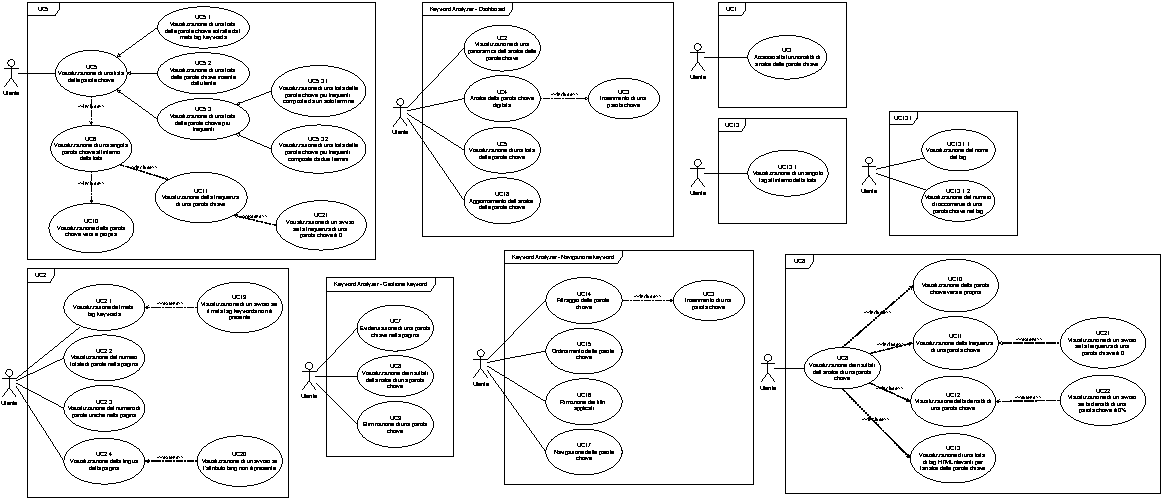
\includegraphics[width=\columnwidth]{usecase/diagrammi_use_case} 
    \caption{Diagrammi dei casi d'uso}
\end{figure}

\begin{usecase}{1}{Accesso alla funzionalità di analisi delle parole chiave}\label{UC1}
    \usecaseactors{Utente.}
    \usecasepre{L'utente ha avviato l'estensione.}
    \usecasedesc{L'utente seleziona la funzionalità di analisi delle parole chiave.}
    \usecasepost{Il sistema mostra la schermata di analisi delle parole chiave.}
\end{usecase}

\begin{usecase}{2}{Visualizzazione di una panoramica dell'analisi delle parole chiave}\label{UC2}
    \usecaseactors{Utente.}
    \usecasepreEnv{
        \begin{itemize}
            \item L'utente ha selezionato la funzionalità di analisi delle parole chiave;
            \item Il sistema è attivo e funzionante.
        \end{itemize}}
    \usecasepost{Il sistema mostra una panoramica dell'analisi delle parole chiave.}
    \usecasesubEnv{
        \begin{itemize}
            \item \hyperref[UC2point1]{UC2.1}: Visualizzazione del meta tag `keywords`;
            \item \hyperref[UC2point2]{UC2.2}: Visualizzazione del numero totale di parole nella pagina;
            \item \hyperref[UC2point3]{UC2.3}: Visualizzazione del numero di parole uniche nella pagina;
            \item \hyperref[UC2point4]{UC2.4}: Visualizzazione della lingua della pagina.
        \end{itemize}}
\end{usecase}

\begin{usecase}{2.1}{Visualizzazione del meta tag `keywords`}\label{UC2point1}
    \usecaseactors{Utente.}
    \usecasepreEnv{\begin{itemize}
        \item L'utente ha selezionato la funzionalità di analisi delle parole chiave;
        \item Il sistema è attivo e funzionante.
    \end{itemize}}
    \usecasepost{Il sistema mostra il meta tag `keywords`.}
    \usecaseextEnv{
        \begin{itemize}
            \item Visualizzazione di un avviso se il meta tag `keywords` non è presente (\hyperref[UC10]{UC10}).
        \end{itemize}}
\end{usecase}

\begin{usecase}{2.2}{Visualizzazione del numero totale di parole nella pagina}\label{UC2point2}
    \usecaseactors{Utente.}
    \usecasepreEnv{\begin{itemize}
        \item L'utente ha selezionato la funzionalità di analisi delle parole chiave;
        \item Il sistema è attivo e funzionante.
    \end{itemize}}
    \usecasepost{Il sistema mostra il numero totale di parole presenti nella pagina.}
\end{usecase}

\begin{usecase}{2.3}{Visualizzazione del numero di parole uniche nella pagina}\label{UC2point3}
    \usecaseactors{Utente.}
    \usecasepreEnv{\begin{itemize}
        \item L'utente ha selezionato la funzionalità di analisi delle parole chiave;
        \item Il sistema è attivo e funzionante.
    \end{itemize}}
    \usecasepost{Il sistema mostra il numero totale di parole uniche presenti nella pagina.}
\end{usecase}

\begin{usecase}{2.4}{Visualizzazione della lingua della pagina}\label{UC2point4}
    \usecaseactors{Utente.}
    \usecasepreEnv{\begin{itemize}
        \item L'utente ha selezionato la funzionalità di analisi delle parole chiave;
        \item Il sistema è attivo e funzionante.
    \end{itemize}}
    \usecasepost{Il sistema mostra la lingua della pagina.}
\end{usecase}

\begin{usecase}{3}{Inserimento di una parola chiave}\label{UC3}
    \usecaseactors{Utente.}
    \usecasepreEnv{\begin{itemize}
        \item L'utente ha selezionato la funzionalità di analisi delle parole chiave;
        \item Il sistema è attivo e funzionante.
    \end{itemize}}
    \usecasedesc{L'utente digita una parola chiave da analizzare.}
    \usecasepost{Il sistema mostra la parola chiave inserita dall'utente nell'apposito campo di testo.}
\end{usecase}

\begin{usecase}{4}{Inserimento di una parola chiave}\label{UC4}
    \usecaseactors{Utente.}
    \usecasepreEnv{\begin{itemize}
        \item L'utente ha selezionato la funzionalità di analisi delle parole chiave;
        \item Il sistema è attivo e funzionante.
    \end{itemize}}
    \usecasedesc{Il sistema esegue l'analisi di una parola chiave scelta dall'utente.}
    \usecasepost{Il sistema aggiunge la parola chiave analizzata alla lista delle keyword.}
    \usecaseincEnv{\begin{itemize}
        \item Inserimento di una parola chiave (\hyperref[UC3]{UC3}).
    \end{itemize}}
\end{usecase}

\begin{usecase}{5}{Visualizzazione di una lista delle parole chiave}\label{UC5}
    \usecaseactors{Utente.}
    \usecasepreEnv{\begin{itemize}
        \item L'utente ha selezionato la funzionalità di analisi delle parole chiave;
        \item Il sistema è attivo e funzionante.
    \end{itemize}}
    \usecasepost{Il sistema mostra una lista delle parole chiave.}
    \usecasesubEnv{
        \begin{itemize}
            \item \hyperref[UC5point1]{UC5.1}: Visualizzazione di una lista delle parole chiave estratte dal meta tag `keywords`;
            \item \hyperref[UC5point2]{UC5.2}: Visualizzazione di una lista delle parole chiave inserite dall'utente;
            \item \hyperref[UC5point3]{UC5.3}: Visualizzazione di una lista delle parole chiave più frequenti.
        \end{itemize}}
    \usecaseincEnv{\begin{itemize}
        \item Visualizzazione di una singola parola chiave (\hyperref[UC6]{UC6}).
    \end{itemize}}
\end{usecase}

\begin{usecase}{5.1}{Visualizzazione di una lista delle parole chiave estratte dal meta tag `keywords`}\label{UC5point1}
    \usecaseactors{Utente.}
    \usecasepreEnv{\begin{itemize}
        \item L'utente ha selezionato la funzionalità di analisi delle parole chiave;
        \item Il sistema è attivo e funzionante.
    \end{itemize}}
    \usecasepost{Il sistema mostra una lista delle parole chiave estratte dal meta tag `keywords`.}
\end{usecase}

\begin{usecase}{5.2}{Visualizzazione di una lista delle parole chiave inserite dall'utente}\label{UC5point2}
    \usecaseactors{Utente.}
    \usecasepreEnv{\begin{itemize}
        \item L'utente ha selezionato la funzionalità di analisi delle parole chiave;
        \item Il sistema è attivo e funzionante.
    \end{itemize}}
    \usecasepost{Il sistema mostra una lista delle parole chiave inserite dall'utente.}
\end{usecase}

\begin{usecase}{5.3}{Visualizzazione di una lista delle parole chiave più frequenti}\label{UC5point3}
    \usecaseactors{Utente.}
    \usecasepreEnv{\begin{itemize}
        \item L'utente ha selezionato la funzionalità di analisi delle parole chiave;
        \item Il sistema è attivo e funzionante.
    \end{itemize}}
    \usecasepost{Il sistema mostra una lista delle parole chiave più frequenti.}
\end{usecase}

\begin{usecase}{6}{Visualizzazione di una singola parola chiave}\label{UC6}
    \usecaseactors{Utente.}
    \usecasepreEnv{\begin{itemize}
        \item L'utente ha selezionato la funzionalità di analisi delle parole chiave;
        \item Il sistema è attivo e funzionante;
        \item È visibile la lista delle parole chiave.
    \end{itemize}}
    \usecasepost{L'utente visualizza una singola parola chiave.}
    \usecaseincEnv{\begin{itemize}
        \item Visualizzazione dei risultati dell'analisi di una parola chiave (\hyperref[UC7]{UC7}).
    \end{itemize}}
\end{usecase}

\begin{usecase}{7}{Visualizzazione dei risultati dell'analisi di una parola chiave}\label{UC7}
    \usecaseactors{Utente.}
    \usecasepreEnv{\begin{itemize}
        \item L'utente ha selezionato la funzionalità di analisi delle parole chiave;
        \item Il sistema è attivo e funzionante.
    \end{itemize}}
    \usecasepost{L'utente visualizza i risultati dell'analisi di una parola chiave.}
    \usecasesubEnv{
        \begin{itemize}
            \item \hyperref[UC7point1]{UC7.1}: Visualizzazione della frequenza di una parola chiave;
            \item \hyperref[UC7point2]{UC7.2}: Visualizzazione della densità di una parola chiave;
            \item \hyperref[UC7point3]{UC7.3}: Visualizzazione di un elenco dei tag in cui dovrebbe essere presente una parola chiave.
        \end{itemize}}
\end{usecase}

\begin{usecase}{7.1}{Visualizzazione della frequenza di una parola chiave}\label{UC7point1}
    \usecaseactors{Utente.}
    \usecasepreEnv{\begin{itemize}
        \item L'utente ha selezionato la funzionalità di analisi delle parole chiave;
        \item Il sistema è attivo e funzionante.
    \end{itemize}}
    \usecasepost{L'utente visualizza la frequenza di una parola chiave.}
\end{usecase}

\begin{usecase}{7.2}{Visualizzazione della densità di una parola chiave}\label{UC7point2}
    \usecaseactors{Utente.}
    \usecasepreEnv{\begin{itemize}
        \item L'utente ha selezionato la funzionalità di analisi delle parole chiave;
        \item Il sistema è attivo e funzionante.
    \end{itemize}}
    \usecasepost{L'utente visualizza la densità di una parola chiave.}
    \usecaseextEnv{\begin{itemize}
        \item Visualizzazione di un avviso se la densità di una parola chiave è troppo alta (\hyperref[UC11]{UC11}).
    \end{itemize}}
\end{usecase}

\begin{usecase}{7.3}{Visualizzazione di un elenco dei tag in cui dovrebbe essere presente una parola chiave}\label{UC7point3}
    \usecaseactors{Utente.}
    \usecasepreEnv{\begin{itemize}
        \item L'utente ha selezionato la funzionalità di analisi delle parole chiave;
        \item Il sistema è attivo e funzionante.
    \end{itemize}}
    \usecasepost{L'utente visualizza un elenco dei tag in cui dovrebbe essere presente una parola chiave.}
    \usecasesubEnv{\begin{itemize}
        \item \hyperref[UC7point3point1]{UC7.3.1}: Visualizzazione di un singolo tag.
    \end{itemize}}
\end{usecase}

\begin{usecase}{7.3.1}{Visualizzazione di un singolo tag}\label{UC7point3point1}
    \usecaseactors{Utente.}
    \usecasepreEnv{\begin{itemize}
        \item L'utente ha selezionato la funzionalità di analisi delle parole chiave;
        \item Il sistema è attivo e funzionante;
        \item L'utente sta visualizzando i risultati dell'analisi di una parola chiave;
        \item È visibile l'elenco dei tag.
    \end{itemize}}
    \usecasepost{L'utente visualizza un singolo tag.}
    \usecasesubEnv{\begin{itemize}
        \item \hyperref[UC7point3point1point1]{UC7.3.1.1}: Visualizzazione del nome del tag;
        \item \hyperref[UC7point3point1point2]{UC7.3.1.2}: Visualizzazione del numero di occorrenze di una parola chiave nel tag.
    \end{itemize}}
\end{usecase}

\begin{usecase}{7.3.1.1}{Visualizzazione del nome del tag}\label{UC7point3point1point1}
    \usecaseactors{Utente.}
    \usecasepreEnv{\begin{itemize}
        \item L'utente ha selezionato la funzionalità di analisi delle parole chiave;
        \item Il sistema è attivo e funzionante.
    \end{itemize}}
    \usecasepost{L'utente visualizza il nome del tag.}
\end{usecase}

\begin{usecase}{7.3.1.2}{Visualizzazione del numero di occorrenze di una parola chiave nel tag}\label{UC7point3point1point2}
    \usecaseactors{Utente.}
    \usecasepreEnv{\begin{itemize}
        \item L'utente ha selezionato la funzionalità di analisi delle parole chiave;
        \item Il sistema è attivo e funzionante.
    \end{itemize}}
    \usecasepost{L'utente visualizza il numero di occorrenze di una parola chiave nel tag.}
    \usecaseextEnv{\begin{itemize}
        \item Visualizzazione di un avviso se il numero di occorrenze di una parola chiave nel tag è inferiore a una certa soglia (\hyperref[UC12]{UC12}).
    \end{itemize}}
\end{usecase}

\begin{usecase}{8}{Evidenziazione di una parola chiave nella pagina}\label{UC8}
    \usecaseactors{Utente.}
    \usecasepreEnv{\begin{itemize}
        \item L'utente ha selezionato la funzionalità di analisi delle parole chiave;
        \item Il sistema è attivo e funzionante.
    \end{itemize}}
    \usecasepost{Il sistema evidenzia graficamente tutte le occorrenze di una parola chiave nella pagina.}
\end{usecase}

\begin{usecase}{9}{Aggiornamento dell'analisi delle parole chiave}\label{UC9}
    \usecaseactors{Utente.}
    \usecasepreEnv{\begin{itemize}
        \item L'utente ha selezionato la funzionalità di analisi delle parole chiave;
        \item Il sistema è attivo e funzionante.
    \end{itemize}}
    \usecasedesc{L'utente aggiorna manualmente l'analisi delle parole chiave per sincronizzarla con eventuali modifiche dinamiche al \gls{domg}.}
    \usecasepost{Il sistema aggiorna l'analisi delle parole chiave.}
\end{usecase}

\begin{usecase}{10}{Visualizzazione di un avviso se il meta tag `keywords` non è presente}\label{UC10}
    \usecaseactors{Utente.}
    \usecasepreEnv{\begin{itemize}
        \item L'utente ha selezionato la funzionalità di analisi delle parole chiave;
        \item Il sistema è attivo e funzionante.
    \end{itemize}}
    \usecasepost{Il sistema mostra un avviso in cui notifica all'utente che il meta tag `keywords` non è presente.}
\end{usecase}

\begin{usecase}{11}{Visualizzazione di un avviso se la densità di una parola chiave è troppo alta}\label{UC11}
    \usecaseactors{Utente.}
    \usecasepreEnv{\begin{itemize}
        \item L'utente ha selezionato la funzionalità di analisi delle parole chiave;
        \item Il sistema è attivo e funzionante.
    \end{itemize}}
    \usecasepost{Il sistema mostra un avviso in cui notifica all'utente che la densità di una parola chiave è troppo alta.}
\end{usecase}

\begin{usecase}{12}{Visualizzazione di un avviso se il numero di occorrenze di una parola chiave nel tag è inferiore a una certa soglia}\label{UC12}
    \usecaseactors{Utente.}
    \usecasepreEnv{\begin{itemize}
        \item L'utente ha selezionato la funzionalità di analisi delle parole chiave;
        \item Il sistema è attivo e funzionante.
    \end{itemize}}
    \usecasepost{Il sistema mostra un avviso in cui notifica all'utente che il numero di occorrenze di una parola chiave nel tag è inferiore a una certa soglia.}
\end{usecase}

\newpage

\section{Tracciamento dei requisiti}
\par I requisiti del progetto, individuati e formalizzati durante il processo di analisi, sono illustrati nelle tabelle \ref{tab:requisiti-funzionali}, \ref{tab:requisiti-qualitativi} e \ref{tab:requisiti-vincolo} secondo la seguente notazione:
\par \textbf{\[R[Tipologia].[Importanza].[Codice]\]} 
\par dove:
\par\vspace{20pt}
\begin{tabular}{@{}ll@{}}
    R = & requisito \\
    \textbf{Tipologia}: & \\
    \quad F = & funzionale \\
    \quad Q = & di qualità \\
    \quad V = & di vincolo/dominio \\
    \textbf{Importanza}: & \\
    \quad O = & obbligatorio \\
    \quad D = & desiderabile \\  
    \quad OP = & opzionale \\
    Codice = & codice numerico univoco \\
\end{tabular}
    
\par\vspace{30pt}

\renewcommand{\arraystretch}{1.5}
\begin{longtable}{p{0.15\textwidth}p{0.55\textwidth}p{0.2\textwidth}}
\caption{Tabella dei requisti funzionali}
\label{tab:requisiti-funzionali} \\
\hline\hline
\textbf{Requisito} & \textbf{Descrizione} & \textbf{Fonti}\\
\endfirsthead

\caption[]{Tabella dei requisiti funzionali (continua)} \\
\hline\hline
\textbf{Requisito} & \textbf{Descrizione} & \textbf{Fonti} \\ 
\endhead

\multicolumn{3}{r}{{Continua nella prossima pagina}} \\ 
\endfoot

\hline
\endlastfoot

\hline
RF.O.1 & L'utente deve poter accedere alla funzionalità di analisi delle parole chiave. & \hyperref[UC1]{UC1} \\
\hline
RF.O.2 & L'utente deve poter visualizzare una panoramica dell'analisi delle parole chiave. & \hyperref[UC2]{UC2} \\
\hline
RF.O.3 & L'utente deve poter visualizzare il meta tag `keywords`. & \hyperref[UC2point1]{UC2.1} \\
\hline
RF.O.4 & L'utente deve poter visualizzare il numero totale di parole nella pagina. & \hyperref[UC2point2]{UC2.2} \\
\hline
RF.OP.5 & L'utente deve poter visualizzare il numero di parole uniche nella pagina. & \hyperref[UC2point3]{UC2.3} \\
\hline
RF.O.6 & L'utente deve poter visualizzare la lingua della pagina. & \hyperref[UC2point4]{UC2.4} \\
\hline
RF.O.7 & L'utente deve poter inserire una parola chiave da analizzare. & \hyperref[UC3]{UC3} \\
\hline
RF.O.8 & L'utente deve poter analizzare una parola chiave. & \hyperref[UC4]{UC4} \\
\hline
RF.O.9 & L'utente deve poter visualizzare una lista delle parole chiave. & \hyperref[UC5]{UC5} \\
\hline
RF.O.10 & L'utente deve poter visualizzare una lista delle parole chiave estratte dal meta tag `keywords`. & \hyperref[UC5point1]{UC5.1} \\
\hline
RF.O.11 & Il sistema deve visualizzare una lista delle parole chiave inserite dall'utente. & \hyperref[UC5point2]{UC5.2} \\
\hline
RF.OP.12 & L'utente deve poter visualizzare una lista delle parole chiave più frequenti. & \hyperref[UC5point3]{UC5.3} \\
\hline
RF.O.13 & L'utente deve poter visualizzare una singola parola chiave. & \hyperref[UC6]{UC6} \\
\hline
RF.O.14 & L'utente deve poter visualizzare i risultati dell'analisi di una parola chiave. & \hyperref[UC7]{UC7} \\
\hline
RF.O.15 & L'utente deve poter visualizzare la frequenza di una parola chiave. & \hyperref[UC7point1]{UC7.1} \\
\hline
RF.O.16 & L'utente deve poter visualizzare la densità di una parola chiave. & \hyperref[UC7point2]{UC7.2} \\
\hline
RF.D.17 & Il sistema deve mostrare un elenco dei tag in cui dovrebbe essere presente una parola chiave. & \hyperref[UC7point3]{UC7.3} \\
\hline
RF.D.18 & L'utente deve poter visualizzare un singolo tag. & \hyperref[UC7point3point1]{UC7.3.1} \\
\hline
RF.D.19 & L'utente deve poter visualizzare il nome del tag. & \hyperref[UC7point3point1point1]{UC7.3.1.1} \\
\hline
RF.D.20 & L'utente deve poter visualizzare il numero di occorrenze di una parola chiave nel tag. & \hyperref[UC7point3point1point2]{UC7.3.1.2} \\
\hline
RF.O.21 & Il sistema deve evidenziare tutte le occorrenze di una parola chiave nella pagina. & \hyperref[UC8]{UC8} \\
\hline
RF.O.22 & L'utente deve poter aggiornare l'analisi delle parole chiave. & \hyperref[UC9]{UC9} \\
\hline
RF.O.23 & Il sistema deve mostrare un avviso se il meta tag `keywords` non è presente. & \hyperref[UC10]{UC10} \\
\hline
RF.O.24 & Il sistema deve mostrare un avviso se la densità di una parola chiave è troppo alta. & \hyperref[UC11]{UC11} \\
\hline
RF.D.25 & Il sistema deve mostrare un avviso se il numero di occorrenze di una parola chiave nel tag è inferiore a una certa soglia. & \hyperref[UC12]{UC12} \\
\hline
RF.O.26 & Il sistema deve evidenziare le parole chiave con colori diversi in base al tag \gls{htmlg} che le racchiude. & Discussione con la Proponente \\
\end{longtable}

\newpage

\renewcommand{\arraystretch}{1.5}
\begin{longtable}{p{0.15\textwidth}p{0.55\textwidth}p{0.2\textwidth}}
\caption{Tabella dei requisti di qualità}
\label{tab:requisiti-qualitativi} \\
\hline\hline
\textbf{Requisito} & \textbf{Descrizione} & \textbf{Fonti}\\
\endfirsthead
    
\caption[]{Tabella dei requisiti di qualità (continua)} \\
\hline\hline
\textbf{Requisito} & \textbf{Descrizione} & \textbf{Fonti} \\ 
\endhead
    
\multicolumn{3}{r}{{Continua nella prossima pagina}} \\ 
\endfoot
    
\hline
\endlastfoot

\hline
RQ.O.1 & La funzionalità di analisi \gls{seog} deve rispettare le linee guida \gls{wcagg} 2.2, livello AA. & Discussione con la Proponente \\
\hline
RQ.OP.2 & L'estensione deve rimanere attiva su tutte le tab. & Discussione con la Proponente \\
\hline
RQ.D.3 & L'utente deve poter aprire e chiudere l'estensione in modo rapido e intuitivo. & Discussione con la Proponente \\
\end{longtable}

\renewcommand{\arraystretch}{1.5}
\begin{longtable}{p{0.15\textwidth}p{0.55\textwidth}p{0.2\textwidth}}
\caption{Tabella dei requisti di vincolo/dominio}
\label{tab:requisiti-vincolo} \\
\hline\hline
\textbf{Requisito} & \textbf{Descrizione} & \textbf{Fonti}\\
\endfirsthead
        
\caption[]{Tabella dei requisiti di vincolo/dominio (continua)} \\
\hline\hline
\textbf{Requisito} & \textbf{Descrizione} & \textbf{Fonti} \\ 
\endhead
        
\multicolumn{3}{r}{{Continua nella prossima pagina}} \\ 
\endfoot
        
\hline
\endlastfoot

\hline
RV.O.1 & La funzionalità di analisi \gls{seog} deve essere resa disponibile tramite \gls{github} (come codice sorgente) o pubblicata su un'altra piattaforma ad accesso pubblico. & Discussione con la Proponente \\
\hline
RV.O.2 & La funzionalità di analisi SEO deve essere integrata all'interno di un'estensione per Chrome & Discussione con la Proponente \\
\end{longtable}

\par\vspace{20pt}

\subsection{Riepilogo}

\begin{table}[H]
\centering
\caption{Tabella di riepilogo dei requisiti}
\label{tab:riepilogo-requisiti}
% MAX 12.5cm
\begin{tabular}{ccccc}
\hline\hline
\textbf{Requisito} & \textbf{Obbligatorio} & \textbf{Desiderabile} & \textbf{Opzionale} & \textbf{Totale} \\ 
\hline
Funzionale & 19 & 5 & 2 & 26 \\
\hline
Di qualità & 1 & 1 & 1 & 3 \\
\hline 
Di vincolo/dominio & 2 & 0 & 0 & 2 \\
\hline
\textbf{Totale} & 22 & 6 & 3 & \textbf{31} \\ 
\hline
\end{tabular}
\end{table}

\newpage

\section{User story}

\renewcommand{\arraystretch}{1.5}
\begin{tabularx}{\textwidth}{lX}
\caption{Tabella delle user story}
\label{tab:user-story} \\
\hline\hline
\textbf{ID} & \textbf{User story}\\
\endfirsthead
    
\caption[]{Tabella delle user story (continua)} \\
\hline\hline
\textbf{ID} & \textbf{User story} \\ 
\endhead
    
\multicolumn{2}{r}{{Continua nella prossima pagina}} \\ 
\endfoot
    
\hline
\endlastfoot

\hline
1 & Come utente, voglio visualizzare una panoramica dell'analisi delle parole chiave, in modo da avere un'idea generale del contenuto della pagina. \\
\hline
2 & Come utente, voglio visualizzare il meta tag `keywords`, in modo da sapere se è presente o meno. \\
\hline
3 & Come utente, voglio visualizzare il numero di parole totali e uniche presenti nella pagina, in modo da valutare la qualità del contenuto in base all'intento. \\
\hline
4 & Come utente, voglio poter inserire manualmente una parola chiave, in modo da analizzare anche quelle non presenti nel meta tag `keywords` o non rilevate automaticamente dal sistema. \\
\hline
5 & Come utente, voglio visualizzare un elenco delle parole chiave analizzate, organizzate per categoria, in modo da facilitare la navigazione. \\
\hline
6 & Come utente, voglio visualizzare la frequenza e la densità di una parola chiave, in modo da capire se il suo utilizzo è eccessivo o appropriato. \\
\hline
7 & Come utente, voglio visualizzare il numero di occorrenze di una parola chiave nei principali tag \gls{htmlg}, in modo da capire se è presente nei punti strategici della pagina. \\
\hline
8 & Come utente, voglio poter visualizzare graficamente tutte le occorrenze di una parola chiave nella pagina, con colori diversi in base al tag HTML che le contiene, in modo da valutarne la distribuzione. \\
\hline
9 & Come utente, voglio poter aggiornare l'analisi delle parole chiave, in modo da sincronizzarla con eventuali modifiche dinamiche al \gls{domg}. \\
\hline
10 & Come utente, voglio che la funzionalità di analisi \gls{seog} sia accessibile a tutti. \\
\end{tabularx}
        %\chapter{Progettazione e codifica}
\label{cap:progettazione-codifica}

\intro{Breve introduzione al capitolo}\\

\section{Tecnologie e strumenti}
\label{sec:tecnologie-strumenti}

Di seguito viene data una panoramica delle tecnologie e strumenti utilizzati.

\subsection*{Tecnologia 1}
Descrizione Tecnologia 1.

\subsection*{Tecnologia 2}
Descrizione Tecnologia 2

\section{Ciclo di vita del software}
\label{sec:ciclo-vita-software}

\section{Progettazione}
\label{sec:progettazione}

\subsubsection{Namespace 1} %**************************
Descrizione namespace 1.

\begin{namespacedesc}
    \classdesc{Classe 1}{Descrizione classe 1}
    \classdesc{Classe 2}{Descrizione classe 2}
\end{namespacedesc}


\section{Design Pattern utilizzati}

\section{Codifica}

        %\chapter{Verifica e validazione}
\label{cap:verifica-validazione}

        %\chapter{Conclusioni}
\label{cap:conclusioni}

\section{Consuntivo finale}

\par Il periodo di stage si è svolto dal 7 aprile al 9 giugno 2025, per un totale di 9 settimane. Rispetto al piano di lavoro standard è stata aggiunta una settimana, interamente dedicata all’analisi delle soluzioni esistenti e alla stesura di una relazione. Nelle prime sei settimane sono state svolte 40 ore di lavoro ciascuna, mentre nelle ultime tre l’impegno è stato di 30 ore settimanali, per un totale complessivo di 330 ore.

\section{Raggiungimento degli obiettivi}

\par Come illustrato nelle tabelle \ref{tab:requisiti-implementazione} e \ref{tab:test-automatici}, tutti i \gls{requisiti} funzionali sono stati soddisfatti, con una copertura del codice e un superamento dei test pari al 100\%. Nella tabella \ref{tab:requisiti-implementazione} sono riportate le classi che hanno contribuito al soddisfacimento di ciascun requisito. Tra i \gls{requisiti} di vincolo, di dominio e di qualità, l’unico obiettivo non raggiunto riguarda l’attivazione automatica dell’estensione su tutte le tab del browser. Questo requisito, previsto nel piano di lavoro e per il quale era stata già progettata l’interfaccia grafica, non è stato implementato per dedicare maggiori risorse al collaudo e all’ottimizzazione delle funzionalità preesistenti.

\section{Conoscenze acquisite}

\par Durante il periodo di stage ho avuto l’opportunità di approfondire i componenti fondamentali per lo sviluppo di un’estensione web: il file \textit{manifest.json}, il \textit{service worker} \textit{(background script)} e il \textit{content script}. In particolare, ho trovato stimolante poter applicare e integrare le conoscenze acquisite durante il percorso accademico - come \gls{api}, \gls{design-pattern}, testing e Chrome DevTools - all’interno di un ambiente di sviluppo moderno, quello delle estensioni.

\vspace{10pt}
\par\noindent Il progetto mi ha permesso di analizzare in profondità il linguaggio \gls{javascript}, che in passato avevo sempre messo in secondo piano rispetto ad \gls{html} e \gls{css}, imparando ad apprezzarne sia le potenzialità che le criticità. Inoltre, ho potuto mettere in pratica le competenze maturate durante il corso di Ingegneria del Software, applicando fin dall’inizio le pratiche di sviluppo in modo attento e consapevole. Questo approccio mi ha aiutato a organizzare il lavoro in modo sostenibile, rispettare le scadenze e comprendere concretamente i vantaggi di una buona progettazione nel lungo periodo, soprattutto nella fase di testing.

\vspace{10pt}
\par\noindent Tra le competenze più significative acquisite durante lo stage, vi è senza dubbio la capacità di integrare nuove funzionalità all’interno di un progetto preesistente, unita alla flessibilità necessaria per adattarsi all’architettura e allo stile definiti da altri sviluppatori. Contribuire a un software non scritto in prima persona ha rappresentato per me una sfida nuova e stimolante, considerando che, nel mio percorso accademico, avevo sempre lavorato a progetti sviluppati “da zero”.

\section{Valutazione personale}

\par Ho trovato questa esperienza estremamente formativa, perché mi ha dato la possibilità di sviluppare un progetto destinato a scenari d’uso concreti, e non esclusivamente orientato alla ricerca teorica, con la consapevolezza del contesto di utilizzo primario. L’estensione, infatti, è pensata come strumento di supporto per la Proponente nella valutazione dei progetti didattici realizzati dagli studenti iscritti al corso di Tecnologie Web. La definizione concreta del contesto di utilizzo mi ha motivato a seguire un modello di sviluppo il più possibile allineato allo “stato dell’arte”, cosa che in passato era avvenuta in modo meno rigoroso o solo parzialmente consapevole. Ritengo che il software realizzato possa costituire una risorsa utile anche per i miei futuri progetti personali.

\vspace{10pt}
\par\noindent Dal punto di vista prettamente teorico, il tirocinio mi ha avvicinato ulteriormente al mondo dell’ottimizzazione \gls{seo}, ambito che avevo già iniziato a esplorare collaborando con una redazione online nella scrittura di blog tramite \gls{wordpress}. Così come rendere i contenuti web accessibili è fondamentale, anche ottimizzarli per migliorarne il posizionamento sui motori di ricerca si è rivelata, grazie a questo progetto, un’attività non solo necessaria ma anche affascinante e intrigante, indipendentemente dal settore digitale di applicazione.

    
        %\appendix
        %\chapter{Appendice A}

\epigraph{Citazione}{Autore della citazione}

    
        \backmatter
        \printglossary[type=\acronymtype, title=Acronimi e abbreviazioni, toctitle=Acronimi e abbreviazioni]
        \printglossary[type=main, title=Glossario, toctitle=Glossario]
    
        \cleardoublepage
\chapter{Bibliografia}

\nocite{*}

% Print book bibliography
\printbibliography[heading=subbibliography,title={Riferimenti bibliografici},type=book]

% Print site bibliography
\printbibliography[heading=subbibliography,title={Siti web consultati},type=online]

    \end{document}
    